\singlespacing

\clearpage

\appendix

\setcounter{table}{0}
\renewcommand{\thetable}{A\arabic{table}}

\section*{Appendix}

\DoToC

\section{FOIA Data}

Our data represent a near census of requests to federal departments, agencies, and sub-agencies. We received records from every department other than the Department of State,\footnote{The Department of State has a notorious FOIA backlog of approximately 10,500 cases. The FOIA office expects to fill our May 2018 request in 2024.} 
and most independent agencies, commissions, boards, executive offices (e.g., the Council on Environmental Quality and U.S. Trade Representative), and pseudo-governmental institutions like Amtrak and the US Export-Import Bank. 

\subsection{Variation in Responses to Identical FOIA Request} Responses to our FOIA requests varied significantly. Most agencies offered logs of congressional correspondence, which record a date, sender, summary of the request, and other information used by agency staff to process and respond to requests. Logs generally include any written requests, as well as many phone and email records. For example, between May 2015 and December 2017, the Department of Justice Office of Administrative Law Judges received 132 emails, 109 telephone calls, and only 54 letters. Between 2007 and 2017, the Postal Regulatory Commission received 100 emails, 30 faxes, 173 letters, and 118 calls. In this paper, we use ``contacts'' and ``letters'' interchangeably to refer to all modes of correspondence. 

Small agencies and regional offices had staff search their email history or provided hand-written records, which we then transcribed. Department Secretary offices generally queried a correspondence tracking database designed to track all correspondence. Still, our FOIA requests to sub-departmental components almost always recovered additional congressional correspondence records missing from central databases. As one central office FOIA officer put it, ``Legislative Affairs is supposed to be the front door for the department, but if somebody knows somebody, well...'' (personal communication, February 21, 2018). Because of such idiosyncratic relationships, capturing correspondence patterns that ``go around'' a Department Secretary's office is key to avoiding erroneous inferences about legislator behavior. For example, when chairs of the Homeland Security committee wrote about immigration enforcement issues, they almost always contacted the Department of Homeland Security (DHS) office of the Executive Secretary, but, at the same time, the Immigration Customs Enforcement (ICE) component of DHS directly received thousands of requests from a different set of legislators. Our systematic data collection ensures that we capture the totality of legislators' behavior.

%%% Ellie: I manually changed the input code here to fit the entire table.  
%\input{tables/FOIA_response.tex}

% TODO replace with this one generated by Appendix.rmd when I get the formatting right

\begin{tabular}{lrrr}
\toprule
Department & Components FOIAed & Records received & N\\
\midrule
Agriculture & 29 & 29 & 9516\\
Commerce & 19 & 18 & 8038\\
Defense & 49 & 13 & 9739\\
Education & 1 & 1 & 4689\\
Energy & 8 & 2 & 6580\\
\addlinespace
Health and Human Services & 15 & 10 & 104145\\
Homeland Security & 14 & 13 & 39633\\
Housing and Urban Development & 2 & 1 & 33968\\
Justice & 23 & 5 & 2611\\
Labor & 22 & 12 & 53341\\
\addlinespace
State & 1 & 0 & 0\\
the Interior & 11 & 8 & 6079\\
the Treasury & 7 & 5 & 23869\\
Transportation & 10 & 7 & 26787\\
Veterans Affairs & 6 & 3 & 77842\\
\addlinespace
Independent Agencies & 77 & 47 & 81053\\
\midrule
\textbf{Total} & \textbf{294} & \textbf{174} & \textbf{487890}\\
\bottomrule
\end{tabular}



\section{Contact Codebook} \label{a:codebook}
\singlespacing
%%% Note: From Ellie. I deleted everything here that we're not using in this paper.  

We provide the following codebook to a team of hand-coders to code each case of Congressional contact with federal agencies and extract information about the legislator. The codebook provides steps to move from raw correspondence logs to data formatted for our analysis.  We also developed subagency-specific coding rules throughout the hand-coding process where certain regular expressions indicated certain types of requests. For example, where documents containing the word ``rulemaking" consistently indicated that a legislator's request involved an agency's proposed rule, we assigned all observations containing the word ``rulemaking" yet uncoded by hand to the ``Policy-Rulemaking" category.\footnote{Hundreds of scripts for processing the raw data from each agency and applying any inductively-generated regular-expression-based coding are available on our GitHub, along with each script's full revision history and all written communication with RAs about processing and coding these data.}

We classify legislator requests into five categories: ``Individual Constituent Service'' (i.e., individual casework or advocacy on behalf of a group such as employees of a company), ``Nonprofit or Local Government Constituent Service'' (e.g., help with a grant application), ``Corporate Constituent Service'' (e.g., help with a specific government contract), ``Corporate Policy'' (policy work explicitly aimed to benefit a specific industry, like tariffs and subsidies), and ``General Policy'' (broader policy work related to legislation, budgets, or rulemaking that is not advocating for an individual constituent or corporatio). We define constituents broadly, so they need not be in a member's district. For example, Representative Tauscher of Wisconsin wrote to the Defense Commissary Agency on behalf of the Jelly Belly Candy Co., based in California. Jelly Belly was then ``given a chance to resolve issues" with their contract. We coded this case as ``Corporate Constituent Service,'' part of our broader measure of constituent service. We also consider constituent service as broader than individual casework. For example, we coded Senator Rubio asking the IRS for special treatment for residents of hurricane-affected parts of Florida as ``Individual Constituent Service.'' We note these ``hard cases'' to illustrate the boundaries of our coding scheme. Most contacts were easily parsed into either individual casework or policy work related to hearings, regulations, and legislation.

\subsection{Congressional Correspondence Log Coding Guidelines}

The first step is to identify the columns that contain the member of Congress (or Committee), the date that the member-initiated correspondence, and the column that best describes the subject. These should be named FROM, DATE, and SUBJECT. 

We aim to classify the subject of correspondence between members of Congress and government agencies. You can do this using keywords (potential keywords in italics below), but it may also require googling subject lines (e.g., what does this acronym mean in this context!?) and inferring why the legislator made the request. Doing so may require identifying a member's relevant policy positions. For example, if the subject is "mining regulations" or "open internet," a member's voting history on related bills or donations from the industry may help us infer if the letter was policy work on behalf of the industry (type 4) or not (type 5). Limiting your search to a date range around the letter date may yield relevant public statements. If you have questions, find something interesting, or, in your efforts to classify a confusing correspondence, you discover information like a related public statement, note it in the NOTES column. In some cases, columns other than the SUBJECT may offer helpful information. This may be difficult at first, but it will get easier. \\

The outcome is a spreadsheet with the first columns being FROM, DATE, SUBJECT, TYPE, CERTAINTY, ALT\_TYPE.\\


Below are five potential codes for the TYPE and three potential codes for your level of CERTAINTY that it is this type. If you are less than Very Certain (i.e., if only Fairly Certain or Toss Up), record your second best guess as ALT\_TYPE; otherwise, leave this column blank. Only leave NOTES if you think it would be helpful for the team to revisit the entry.

TYPE

1 = Personal Service\\

\hfill\begin{minipage}{\dimexpr\textwidth-2cm}
Definition: Individual, non-commercial constituent service.\\
Examples: Help with a government form, passport, visa, back pay, military honor, enlistment, criminal case, request for personal information (e.g., one’s FBI file), disability application, worker compensation, personal complaint, discrimination case, job application, health insurance, financial services complaints, etc.\\
\end{minipage}

2 = Commercial Service - Transactional \\

\hfill\begin{minipage}{\dimexpr\textwidth-2cm}
Definition: Anything related to a specific individual case by a business (including business owners like farmers and consultants).\\ 
General Examples: Help with a grant application, payment, loan, or contract (buying anything from or selling anything to a government agency). Help with an individual case of tax assessment, fine, or regulatory enforcement action. Help with public relations on behalf of a business.\\
Specific Examples: allocation of radio spectrum, a case against a company, tax dispute, contract for the purchase of military surplus, crop insurance distribution, debt settlement, foreclosure assistance, a fine for a law violation, etc. \\
\end{minipage}

3 = Government and Nonprofit Service - Transactional\\

\hfill\begin{minipage}{\dimexpr\textwidth-2cm}
Definition: Same as for (2-Commercial Service), but for municipal or state governments (including cities, counties, etc.) or non-business-oriented nonprofit organizations (i.e., NOT ones that represent an industry or trade association) \\
\end{minipage}

4 = Commercial Service - Policy \\

\hfill\begin{minipage}{\dimexpr\textwidth-2cm}
Definition: Anything applying to a class of commercial activity or businesses (e.g., shipping, airlines, agriculture), including legislation, bills, acts, appropriations, authorizations, etc. \\
General Examples: Authorization of or appropriation to a government program targeted towards a particular industry or industries. Regulation of industry or commercial practice or competition.\\
Specific Examples: Milk prices, insurance or loan eligibility criteria, purchasing policies, crop insurance rates, pollution criteria, classification of products for trade or taxation, conservation appropriation, worker visa types, restrictions, or caps, etc.\\
\end{minipage}
 
5 = Policy Work - NOT in the service of any individual, business, or specific industry.\\

\hfill\begin{minipage}{\dimexpr\textwidth-2cm}
Examples of Policy Work: 
 \begin{tight_itemize} 
 \item Lawmaking 
\item Request for policy-relevant information. This includes prospective legislation, legislation under consideration, or already implemented legislation that requires oversight.  
\item Oversight
\item Committee requesting a report or testimony at a hearing
\item Requesting clarity on an agency rule
\item Lobbying administrative policy
\item Agency rulemaking with non-commercial implications (comments on agency rulemaking may often be (3)) 
\item Political work
\item Meeting with organized constituent groups (e.g., workers, people with disabilities, environmentalists) about policy (meetings with industry groups generally fall under (4)).
\item Media requests
 \end{tight_itemize} 
\end{minipage}
\bigskip


6 = Other \\

\hfill\begin{minipage}{\dimexpr\textwidth-2cm}
	Suggest a new category in the NOTES column only if you cannot fit it under 1-4. For example, requesting dirt on one's political opponents could be called "partisan" as none of the above. Other specific types: thank you (for thank you notes with no other information), congratulations (for congratulatory correspondence on appointments or retirements with no other information), family member (for correspondence on behalf of a family member) \\
\end{minipage}

\clearpage


\section{Additional Models} \label{s:appendix_models}

\subsection{Interpreting Experence Effects }

In Section \ref{s:tenure}, we draw inferences about the effects of legislator experience from a within-district design, showing that new legislators provide less constituency service. The within-legislator design shows results consistent with this conclusion. However, we interpret indicator variables for years of experience in the within-legislator design with caution given the complexity of this model with time shocks and experience increasing in time, which has the potential to cause identification issues in interpreting the estimates for years of experience. Including years of experience as a control is appropriate and important for correctly chair effects, which are clearly identified in these models.  

If we interpret this alternative measure of experience as identified, it shows further support for the conclusions of the within-district models. Legislators make significantly fewer requests to agencies in their first year than they do the following year. Subsequent increases are less significant.  

We estimate that the experience gained between the first and second year in Congress causes an increase of 0.24 requests \textit{per agency}. The experience gained between the first and seventh years causes an increase of 0.51 per agency. Across all \input{tables/n_agencies} agencies in these data, this represents an increase of approximately 46 additional requests per year, 45.5\% of the average number of requests per year in our data. There is a smaller increase after the second year. The experience gained between the second and seventh year causes an increase of 0.28 per agency, an increase of approximately 25 additional requests per year, 24.5\% of the average number of requests per year in our data.

\begin{figure}[hbt!]
\centering
\caption{Predicted Number of Total Letters (Within Legislator Difference in Differences) 2007-2018} \label{f:m-total-predicted-time}
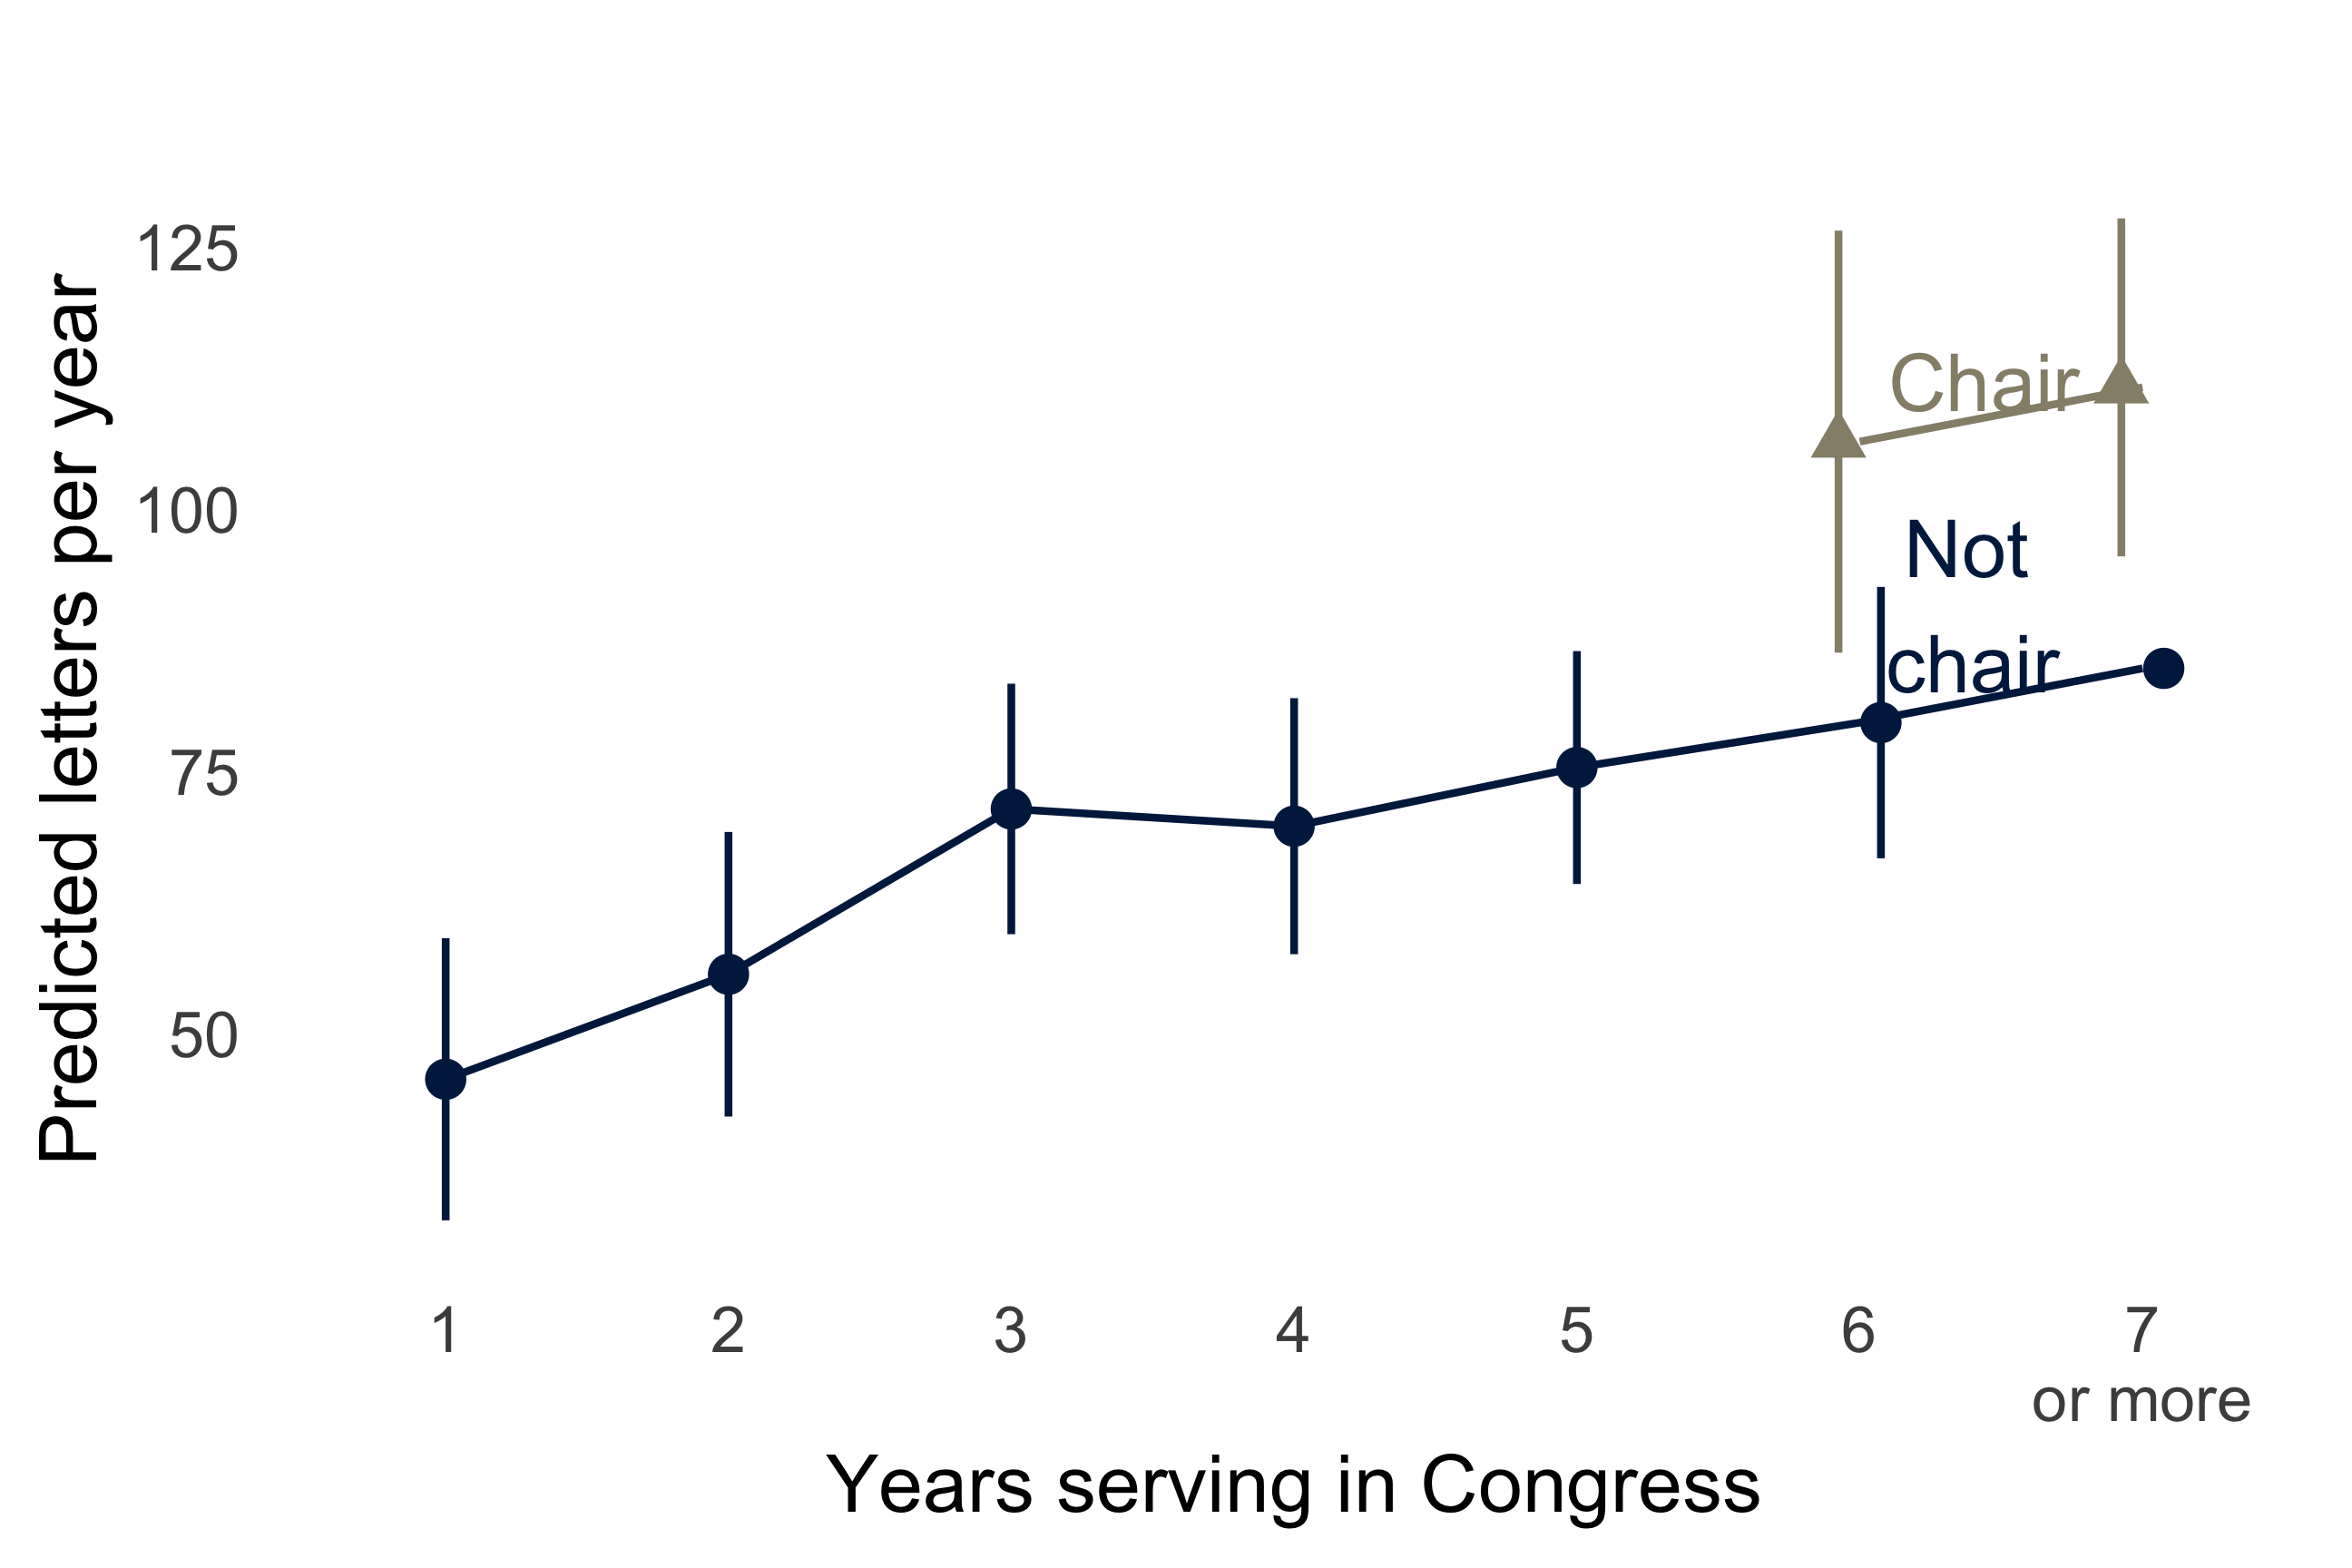
\includegraphics[width = .8\textwidth]{figs/m-total-predicted-4}
\end{figure}

Figure \ref{f:m-total-predicted-time} shows the predicted total number of letters in Congress and committee chair status (comparing predictions for counterfactuals where the same legislator did and did not receive a chairmanship in their sixth year).\footnote{Predictions are based on a legislator-agency pair where (1) the legislators' average annual contacts equaled the overall average, (2) the legislators' number of contacts with the agency equal the average received by that agency, (3) and the agency received an average number of letters.} 


Figure \ref{f:m-total-predicted-time} uses the coefficients in legislators' first six years in office from Table \ref{t:models_total}. The reference group is representatives who have served longer than six years.\footnote{Interpreting these coefficients requires that we assume the effects of tenure and committee assignment are linearly separable. This assumption is reasonable because most legislators do not become chairs, ranking members, or join prestige committees in their first six years, and almost none in their first two years.} 

The first column of Table \ref{t:models_total} shows large cross-sectional differences: legislators in their first year make fewer contacts than more experienced legislators. First-year legislators make approximately 0.255 fewer requests per agency than legislators in their seventh year or beyond. This difference shrinks in the second year and then is mostly gone. But we advise caution in interpreting the differences in Column 1 because they conflate the effect of increased experience with other characteristics that may correlate with whether a legislator remains in office and, thus whether we observe them in later years.   

To account for possible differences in legislators who obtain different levels of tenure, the second column of Table \ref{t:models_total} estimates the difference-in-differences specification in Equation \ref{e:diff1}. The tenure coefficients show that legislators provide less constituency service in their first year in office. As they acquire experience, they make more requests to federal agencies. In their first year in office, legislators provide 21.33 (\input{tables/n_agencies} $\times$ (.512 - .275)) fewer requests per agency than legislators in their second year and 29.07 (\input{tables/n_agencies} $\times$ (.512 - .189)) fewer requests than legislators in their third year---both differences are statistically significant at conventional levels. The overall increase in levels of constituency service from a legislator's first to third year is similar in size to the increase that comes from becoming a member of the oversight committee. Once legislators enter their fourth year, their behavior no longer differs from more experienced legislators. We find small and statistically insignificant differences for legislators in their fourth through sixth years. As legislators acquire experience and build their office's organizational capacity in their first two years, they make more contacts with federal agencies.  

As with the analysis of committee prestige, the findings in Table \ref{t:models_total} are robust to alternative specifications. Despite the difference-in-difference design, we might still be concerned that the set of legislators who served a third year differs from those who served a first year. If this were the case, our findings would result from both the experience and a selection effect due to House members who win reelection, a potential indication that they are better able to perform the job than other legislators. To address the potentially different samples each year, the third column of Table \ref{t:models_total} assesses the changes in the number of contacts of federal agencies for legislators who serve for at least three years. The pattern is similar: legislators initially provide less constituency service in their first two years than in subsequent years. Column 4 in Table \ref{t:models_total} shows that the results are robust to analyzing $\log(Y_{ijt} + 1)$, ensuring that our results are not because of outliers. Additional models below estimate the same models as Table \ref{t:models_total} on hand-coded subsets of the data, showing similar results. 


 




\subsection{Constituency Service Only}

\begin{table}[hbt!]
\caption{The Effect Experience and Institutional Power on Constituency Service} \label{t:models_con}
\begin{minipage}{\textwidth}
\begin{center}
\small
\begin{tabular}[t]{lcccc}
\toprule
  & (1) & (2) & (3) & (4)\\
\midrule
\textbf{Dependent Variable} & \textbf{Count} & \textbf{Count} & \textbf{Count} & \textbf{Log(Count+1)}\\
\midrule
Committee Chair & \num{0.302} & \num{0.040} & \num{0.044} & \num{0.012}\\
 & (\num{0.108}) & (\num{0.064}) & (\num{0.064}) & (\num{0.007})\\
Ranking Member & \num{0.503} & \num{0.054} & \num{0.070} & \num{0.012}\\
 & (\num{0.108}) & (\num{0.067}) & (\num{0.067}) & (\num{0.007})\\
Prestige Committee & \num{0.321} & \num{0.031} & \num{0.025} & \num{0.013}\\
 & (\num{0.049}) & (\num{0.036}) & (\num{0.036}) & (\num{0.007})\\
First Year & \num{-0.138} & \num{-0.276} & \num{-0.265} & \num{-0.059}\\
 & (\num{0.040}) & (\num{0.055}) & (\num{0.054}) & (\num{0.008})\\
Second Year & \num{0.009} & \num{-0.128} & \num{-0.142} & \num{-0.019}\\
 & (\num{0.046}) & (\num{0.053}) & (\num{0.052}) & (\num{0.008})\\
Third Year & \num{0.030} & \num{-0.070} & \num{-0.088} & \num{-0.011}\\
 & (\num{0.047}) & (\num{0.047}) & (\num{0.046}) & (\num{0.007})\\
Fourth Year & \num{0.061} & \num{-0.055} & \num{-0.072} & \num{-0.006}\\
 & (\num{0.052}) & (\num{0.046}) & (\num{0.045}) & (\num{0.006})\\
Fifth Year & \num{0.001} & \num{-0.069} & \num{-0.064} & \num{-0.011}\\
 & (\num{0.044}) & (\num{0.034}) & (\num{0.033}) & (\num{0.005})\\
Sixth Year & \num{0.070} & \num{0.008} & \num{0.018} & \num{-0.004}\\
 & (\num{0.056}) & (\num{0.044}) & (\num{0.043}) & (\num{0.005})\\
\midrule
Majority & \checkmark & \checkmark & \checkmark & \checkmark\\
Presidents` Party & \checkmark & \checkmark & \checkmark & \checkmark\\
All Legislators & \checkmark & \checkmark &  & \checkmark\\
Served At Least 2nd Term &  &  & \checkmark & \\
Observations & \num{412111} & \num{412111} & \num{388997} & \num{412111}\\
Year x Agency FE & \checkmark & \checkmark & \checkmark & \checkmark\\
Legislator x Agency FE &  & \checkmark & \checkmark & \checkmark\\
\bottomrule
\multicolumn{5}{l}{\rule{0pt}{1em}\footnotesize Robust standard errors in parentheses, clustered by legislator.}\\
\end{tabular}
 % this one is from replication.rmd
\end{center}
\footnotetext{This table shows how the number of contacts hand-coded as constituecy service changes as legislators acquire more expiernece and power in Congress. Column 1 shows the average differences across committee assignments and years in Congress. Column 2 presents the difference-in-differences estimates. Column 3 subsets to legislators who serve at least 3 years in Congress. Column 4 takes the Log of the counts + 1 as the dependent variable.}
\end{minipage}
\end{table}

Table \ref{t:models_con} is identical to Table \ref{t:models_total} except that we subset the data to only legislator requests hand-coded as constituency service. 
Column 2 of Table \ref{t:models_con} provides the estimated effects from the difference-in-differences specification in Equation \ref{e:diff1}. More experience increases the level of constituency service that legislators provide. The effect of being a committee chair is positive but not significant at the .05 level. We estimate that the experience gained between the first and second year in Congress causes an increase of 0.02 requests \textit{per agency}. The experience gained between the first and seventh year causes an increase of 0.21 per agency. Across all 92 agencies, this represents an increase of approximately 19 additional requests per year, 21.9\% of the average requests per year in our data. There is a smaller increase after the second year. The experience gained between the second and seventh year causes an increase of 0.19 per agency, an increase of approximately 17 additional requests per year, 19.6\% of the average requests per year in our data.


\begin{figure}[hbt!]
\centering
\caption{Predicted Number of Constituency Service Requests} \label{f:m-con-predicted}
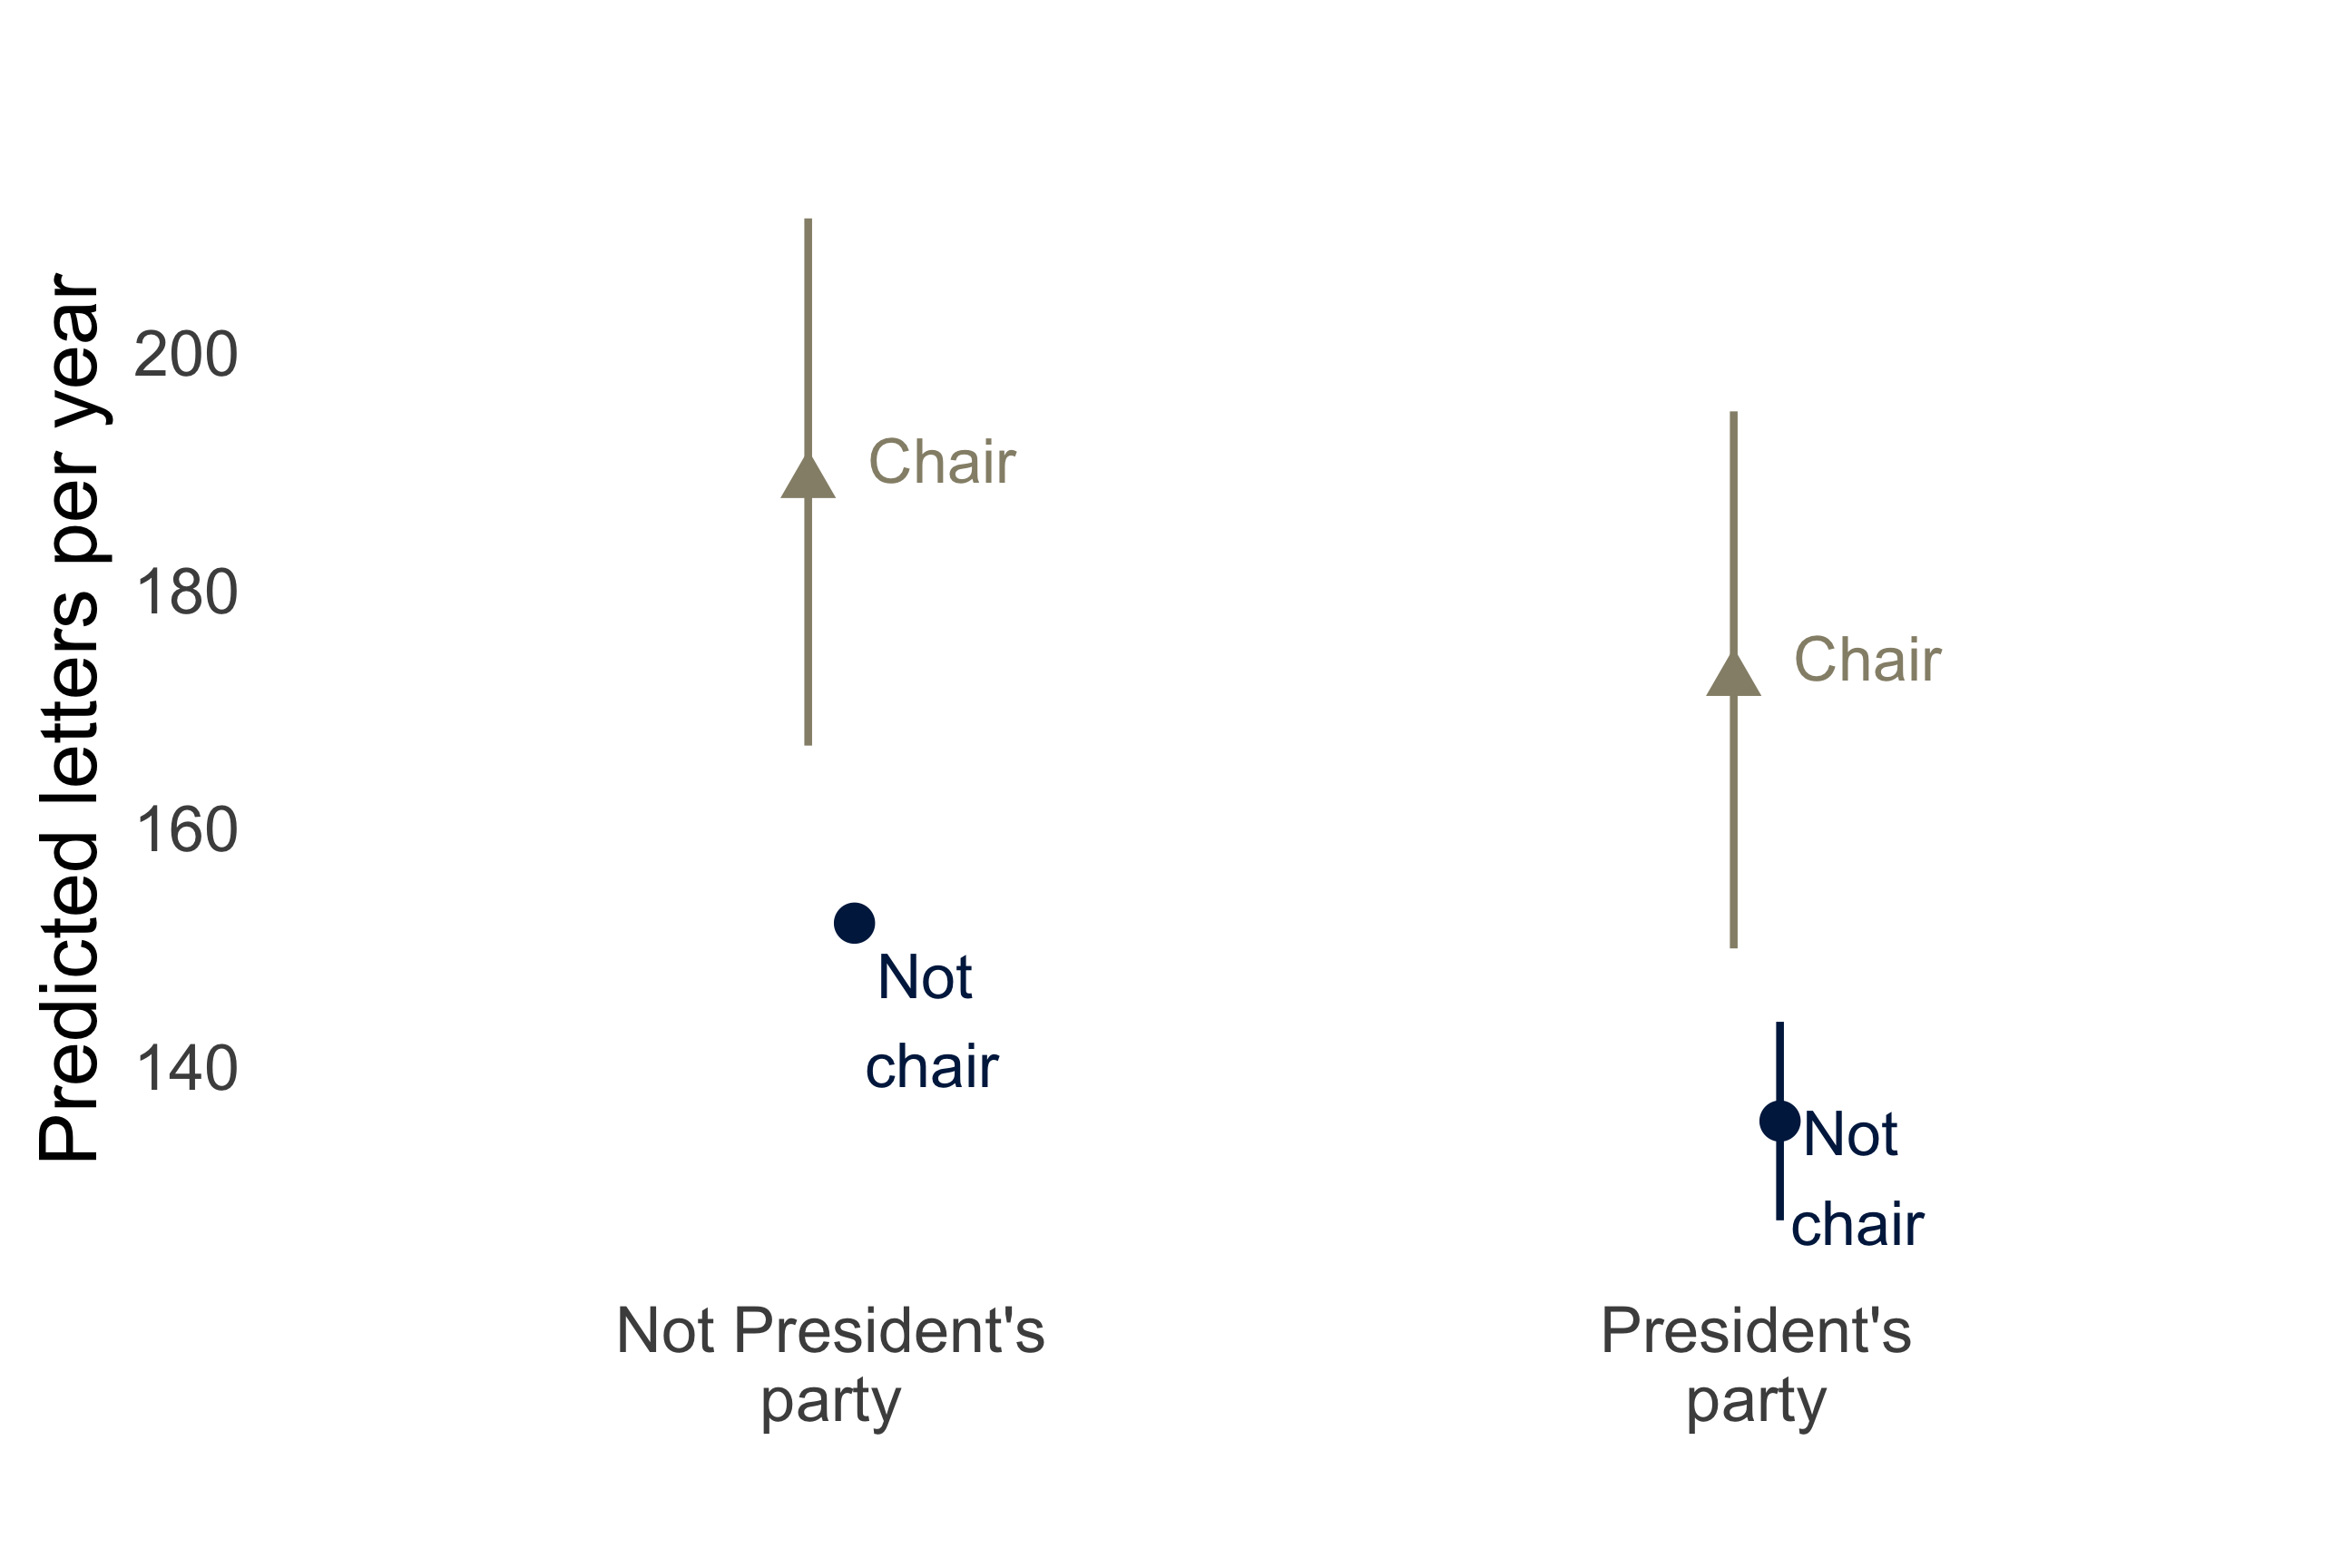
\includegraphics[width = .49\textwidth]{figs/m-con-predicted-1}
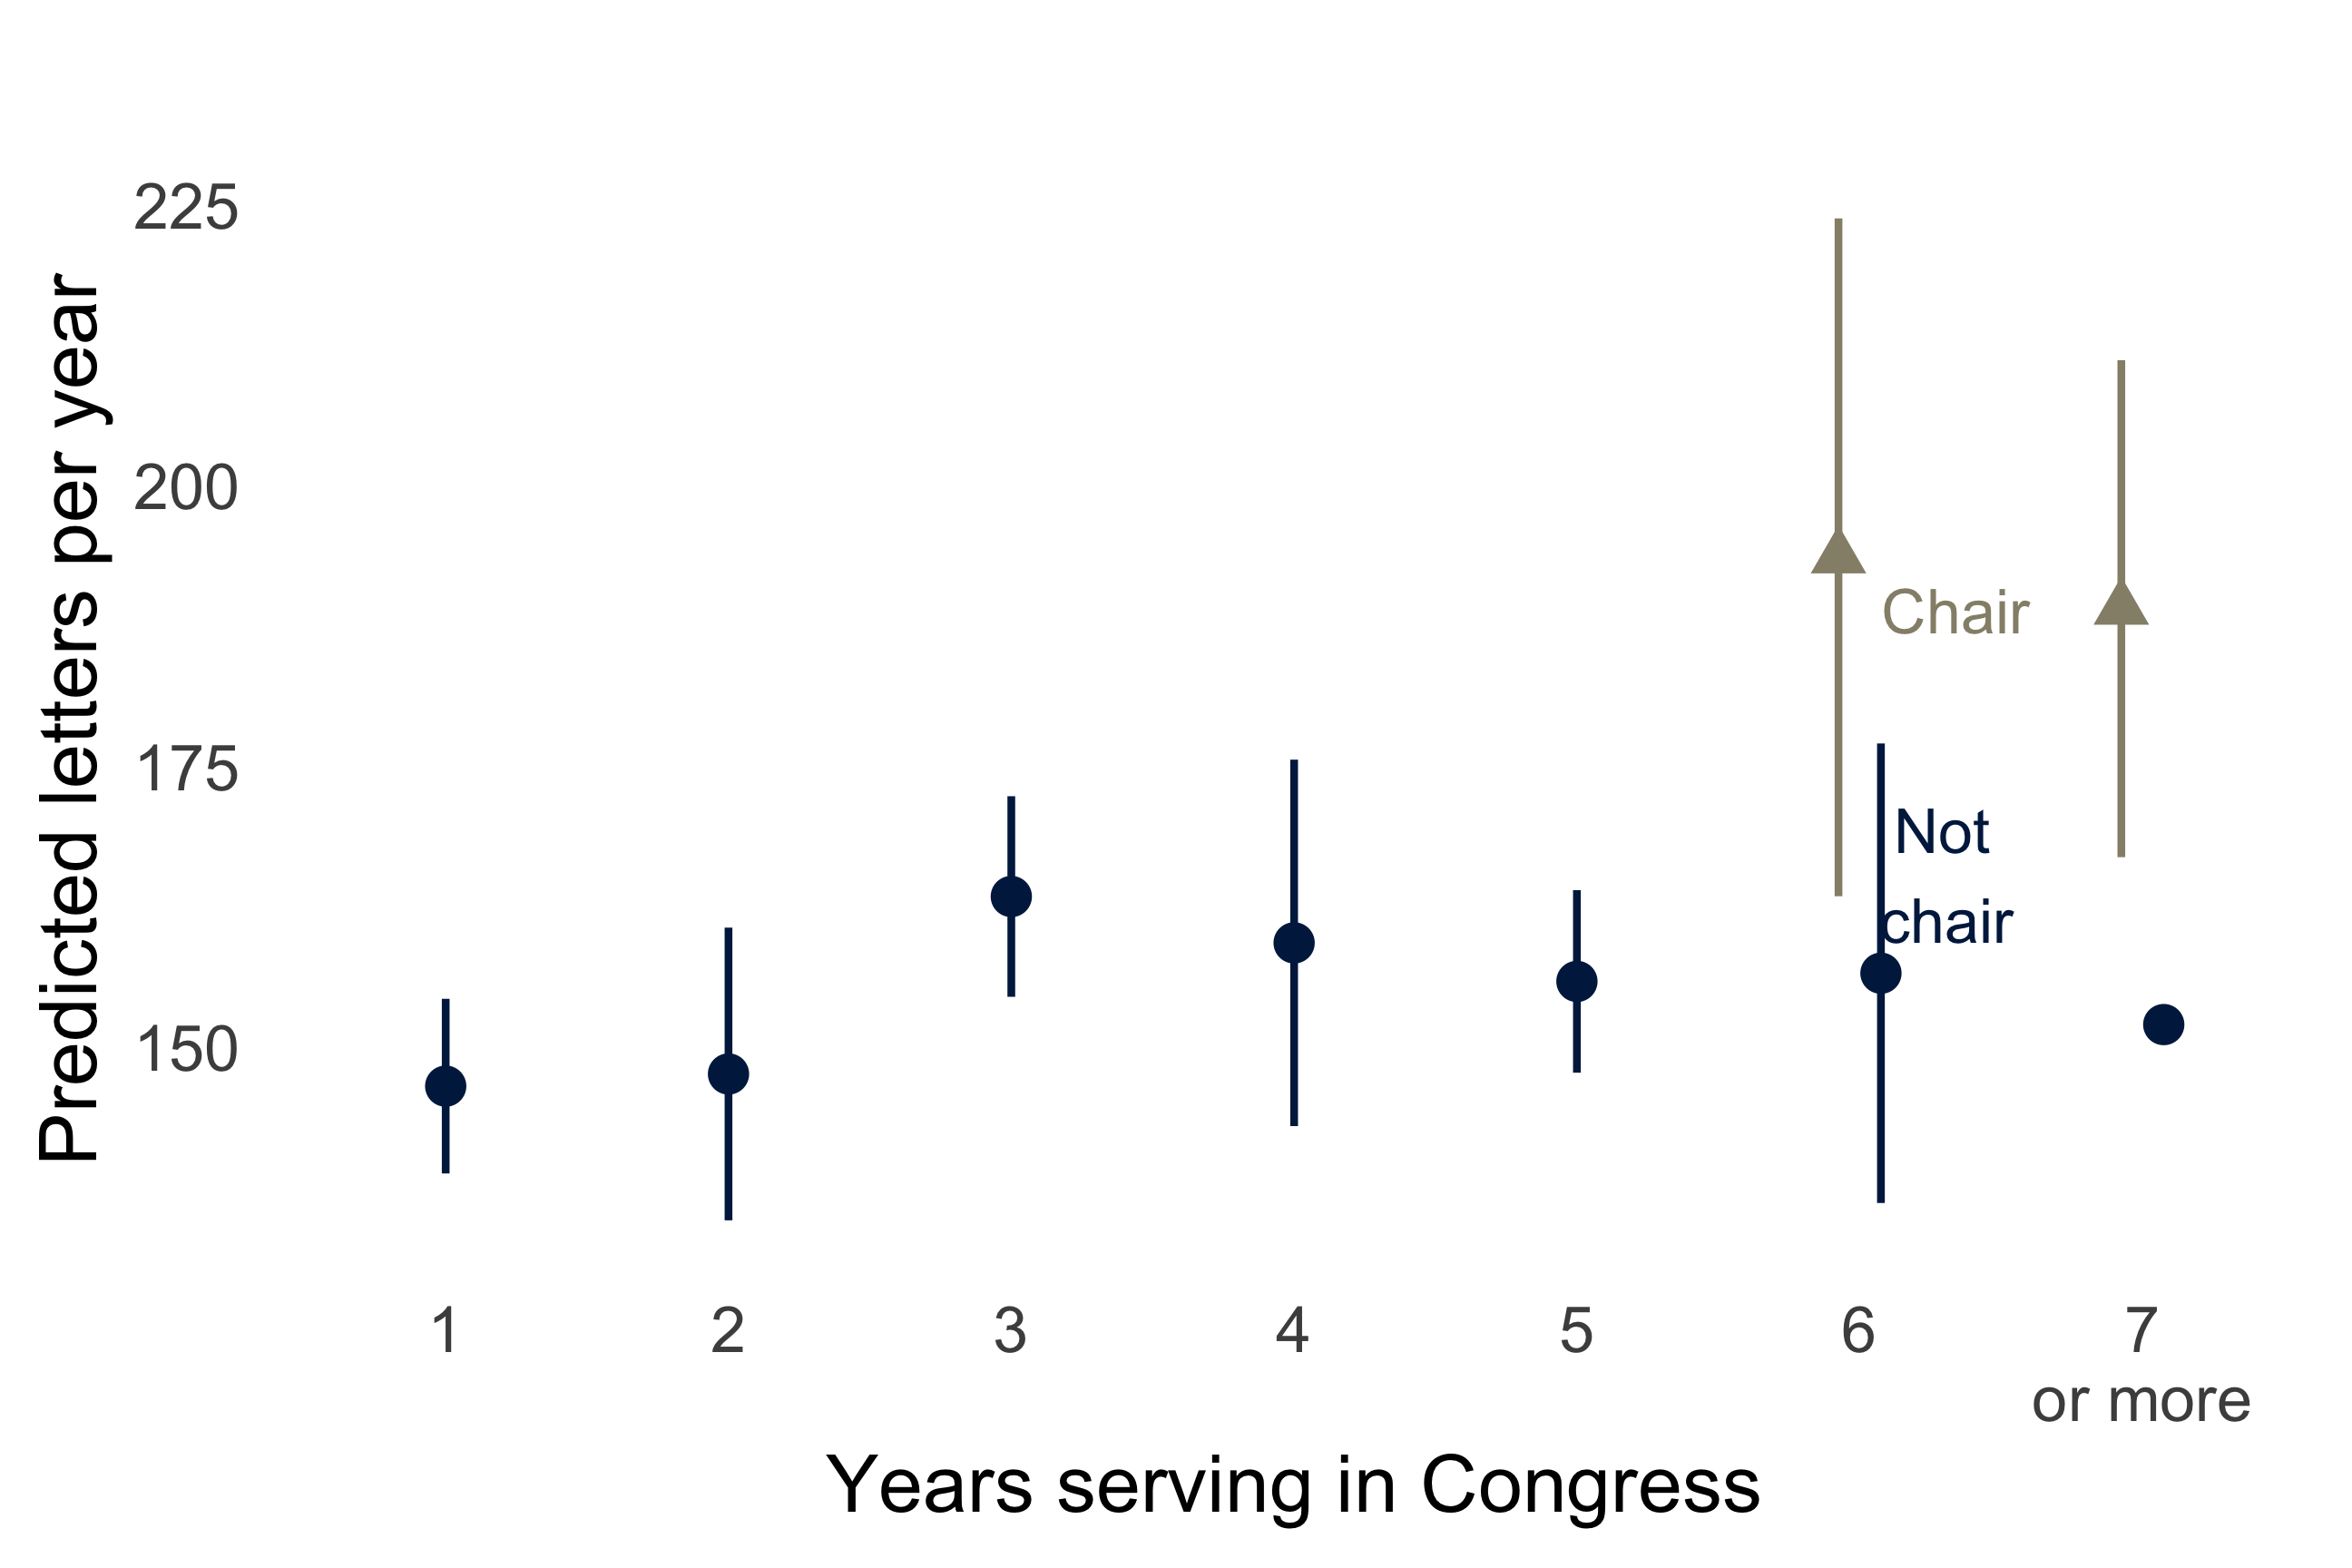
\includegraphics[width = .49\textwidth]{figs/m-con-predicted-2}
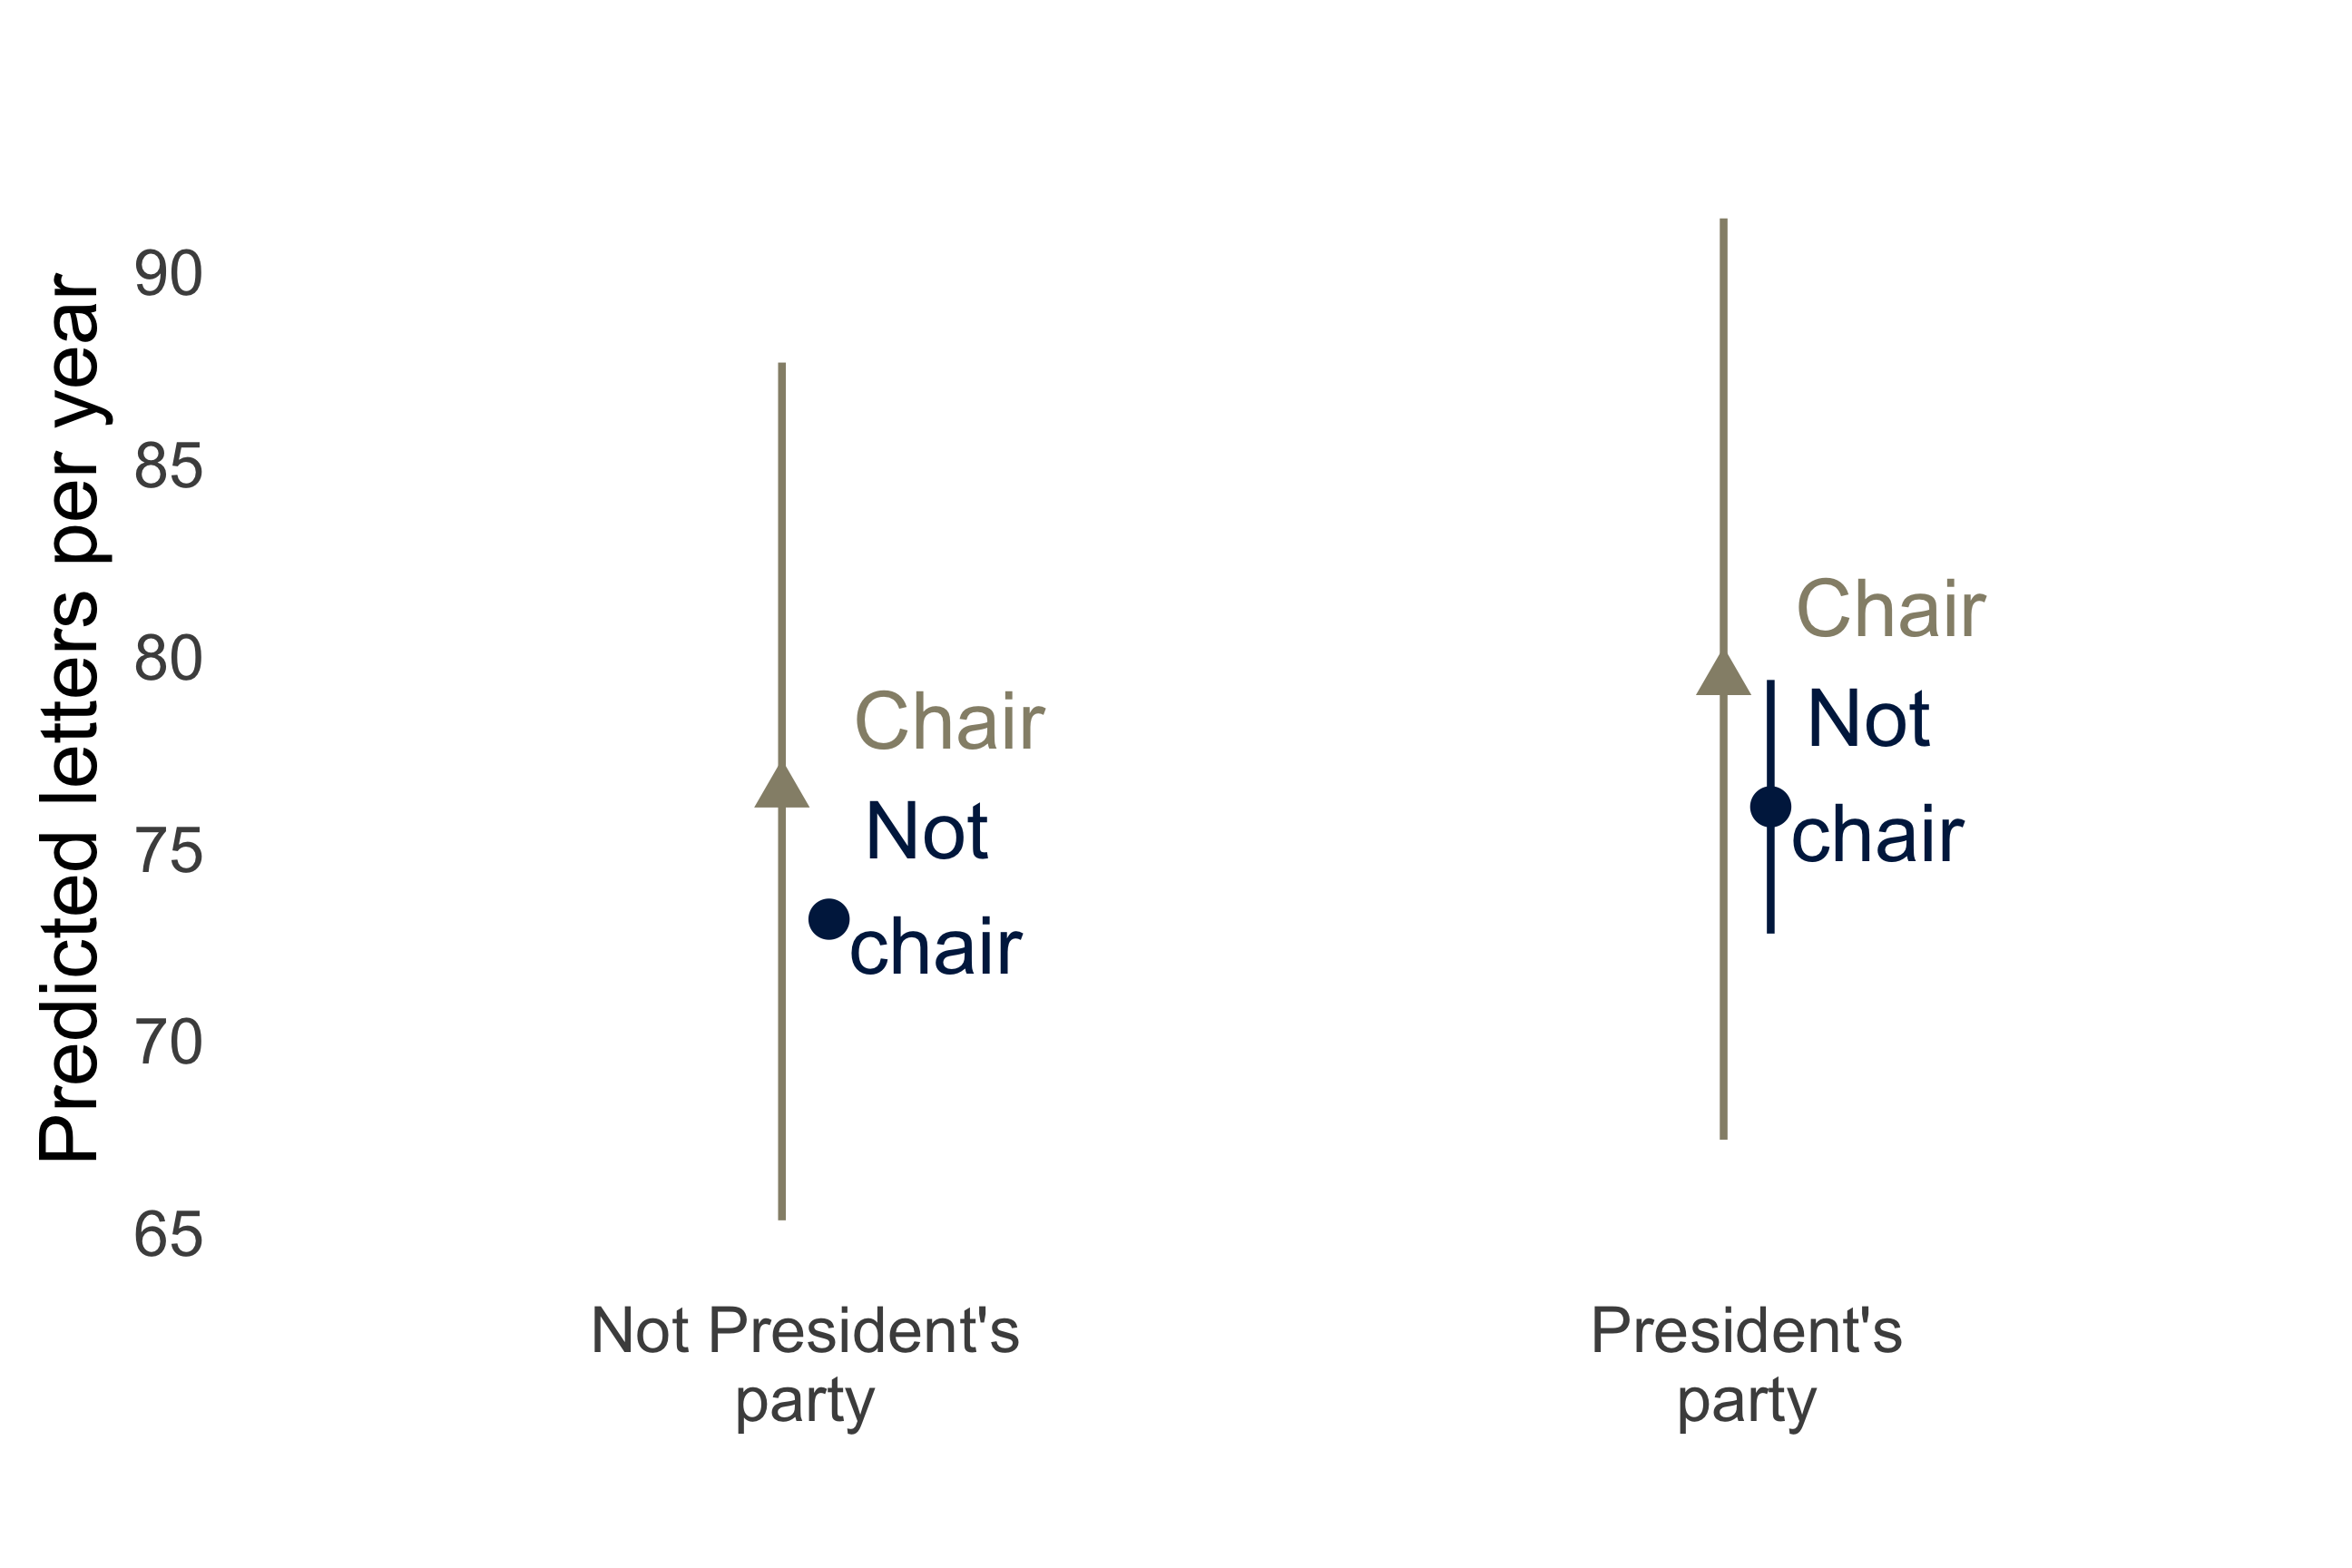
\includegraphics[width = .49\textwidth]{figs/m-con-predicted-3}
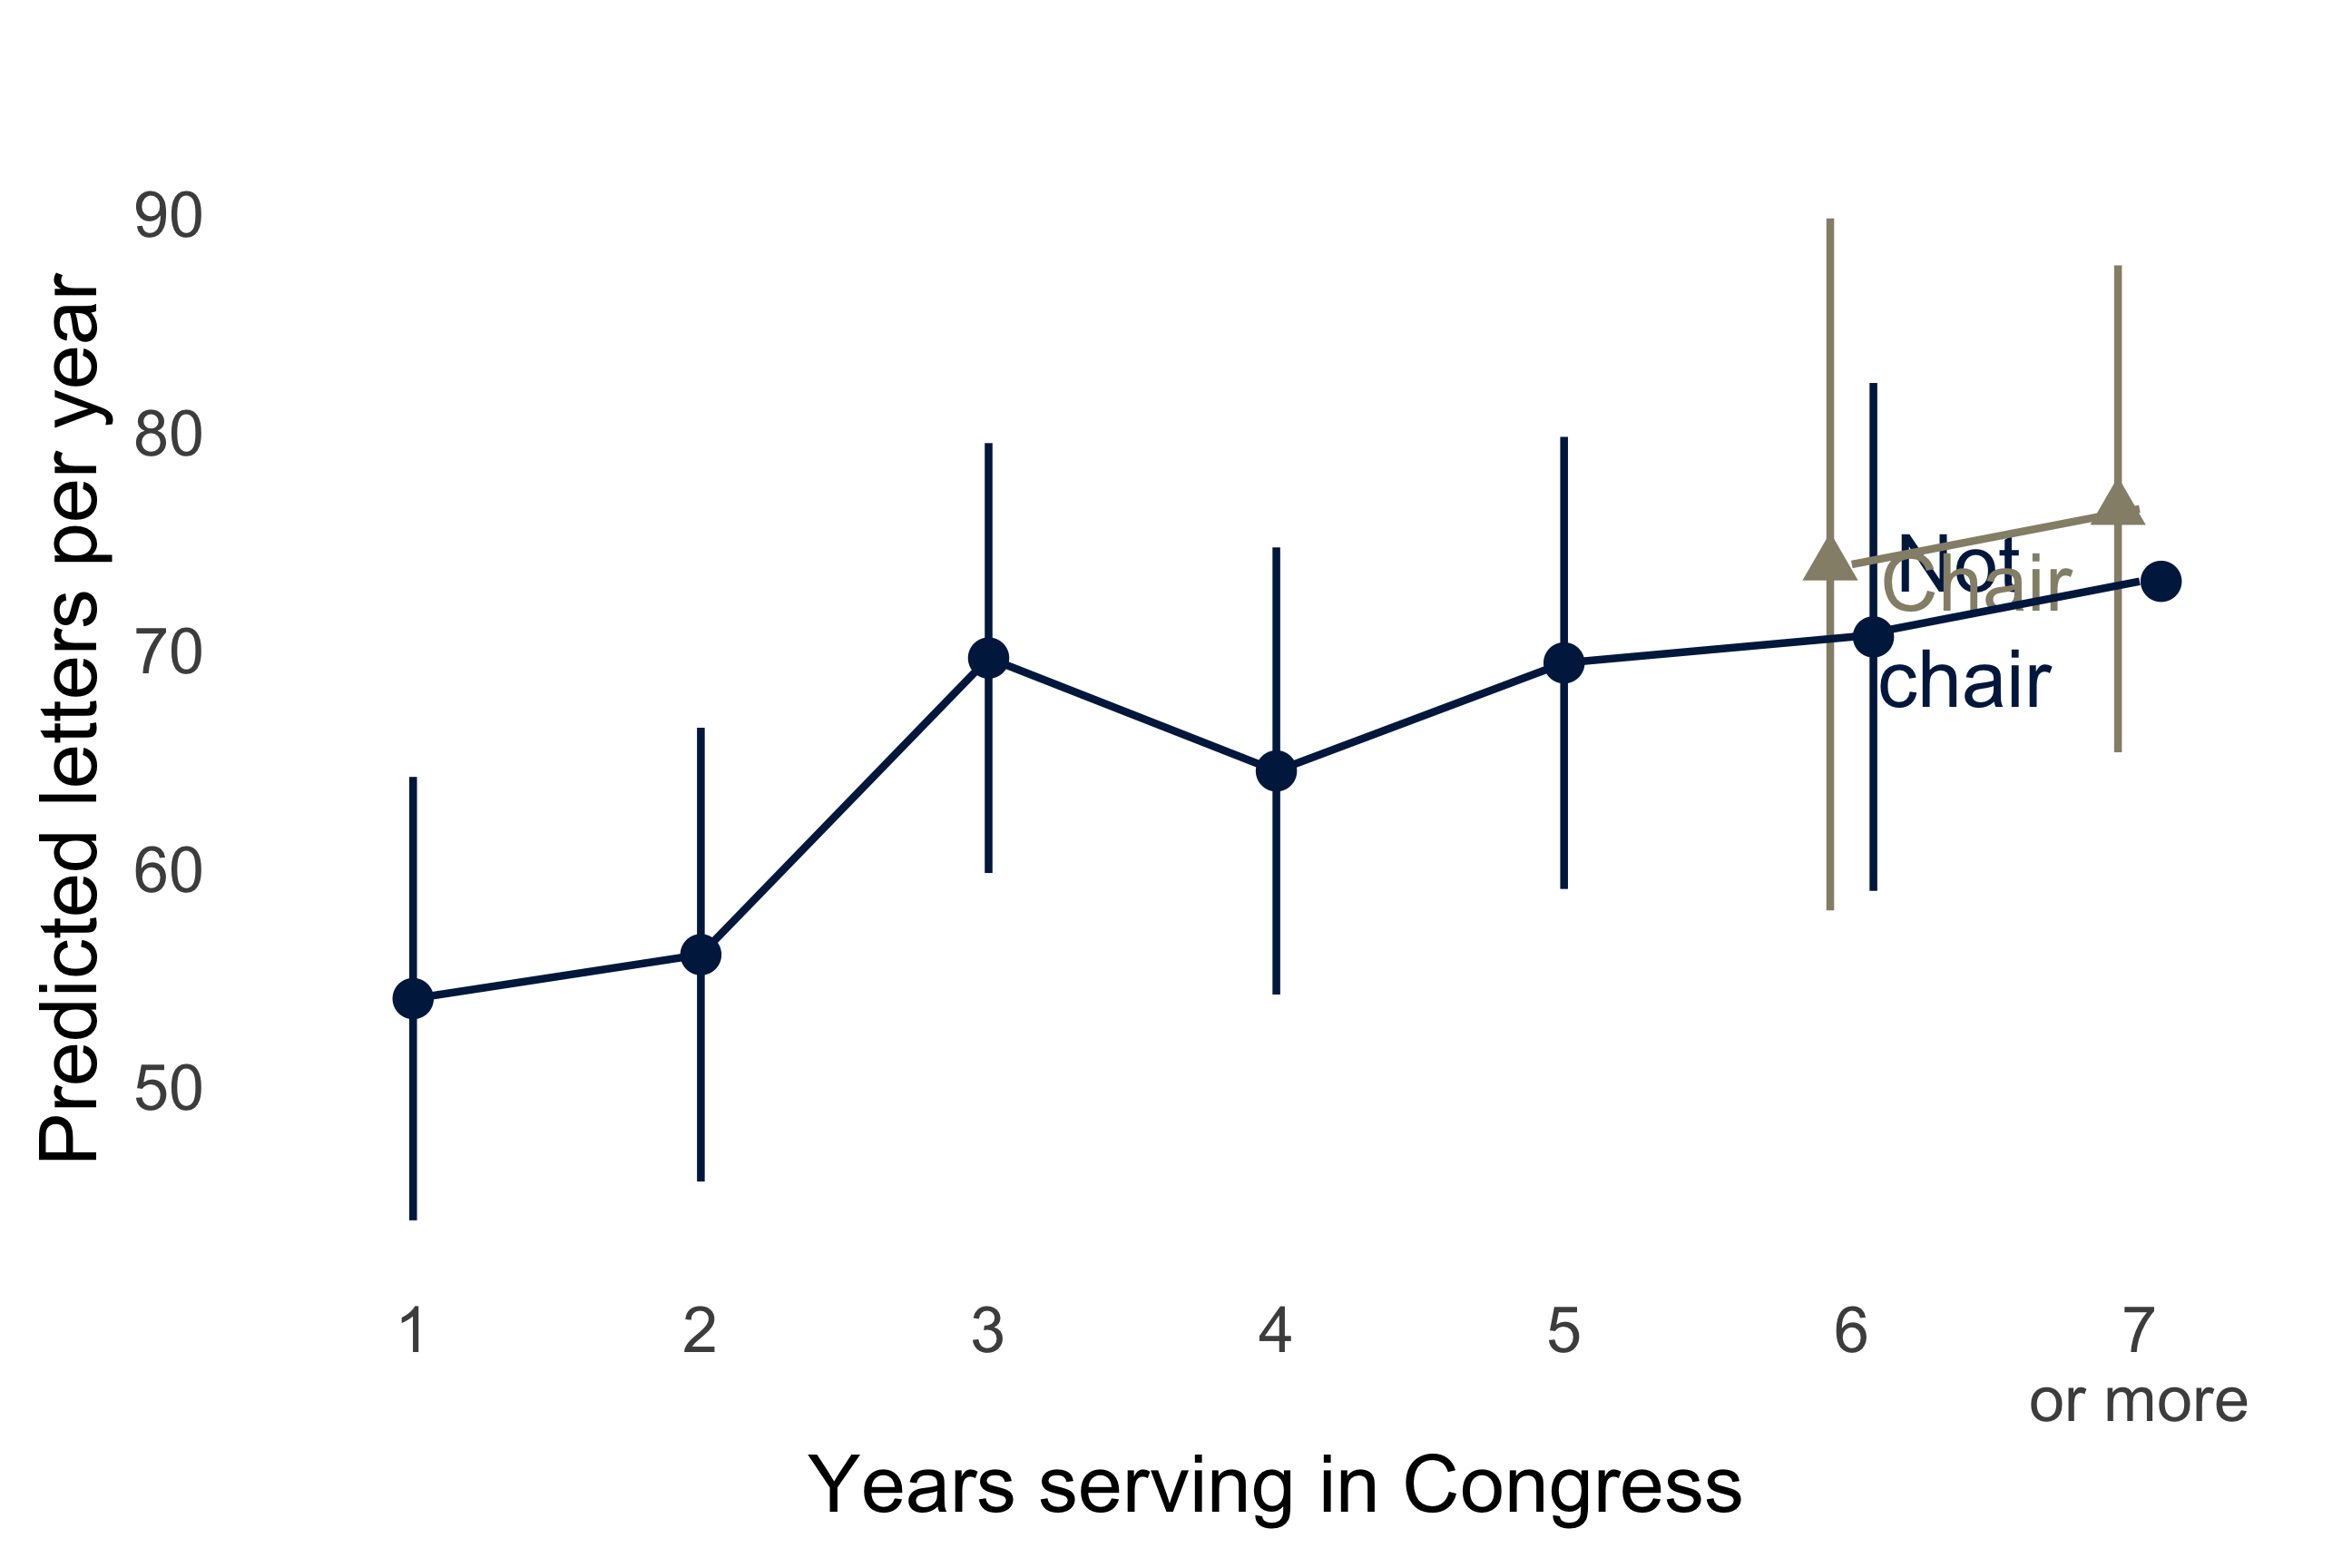
\includegraphics[width = .49\textwidth]{figs/m-con-predicted-4}

\end{figure}

\subsection{Policy Work Only}

\begin{table}[hbt!]
\caption{The Effect Experience and Institutional Power on Policy Work} \label{t:models_policy}
\begin{minipage}{\textwidth}
\begin{center}
\small
\begin{tabular}[t]{lcccc}
\toprule
  & (1) & (2) & (3) & (4)\\
\midrule
\textbf{Dependent Variable} & \textbf{Count} & \textbf{Count} & \textbf{Count} & \textbf{Log(Count+1)}\\
\midrule
Committee Chair & \num{0.199} & \num{0.158} & \num{0.159} & \num{0.036}\\
 & (\num{0.027}) & (\num{0.034}) & (\num{0.034}) & (\num{0.007})\\
Ranking Member & \num{0.145} & \num{0.090} & \num{0.092} & \num{0.025}\\
 & (\num{0.028}) & (\num{0.024}) & (\num{0.024}) & (\num{0.005})\\
Prestige Committee & \num{0.049} & \num{0.031} & \num{0.031} & \num{0.010}\\
 & (\num{0.009}) & (\num{0.010}) & (\num{0.010}) & (\num{0.003})\\
First Year & \num{-0.076} & \num{-0.076} & \num{-0.070} & \num{-0.030}\\
 & (\num{0.007}) & (\num{0.016}) & (\num{0.016}) & \vphantom{1} (\num{0.004})\\
Second Year & \num{-0.045} & \num{-0.042} & \num{-0.040} & \num{-0.018}\\
 & (\num{0.007}) & (\num{0.016}) & (\num{0.016}) & (\num{0.004})\\
Third Year & \num{-0.042} & \num{-0.031} & \num{-0.033} & \num{-0.013}\\
 & (\num{0.008}) & (\num{0.013}) & (\num{0.013}) & (\num{0.004})\\
Fourth Year & \num{-0.021} & \num{-0.011} & \num{-0.013} & \num{-0.006}\\
 & (\num{0.009}) & (\num{0.013}) & (\num{0.013}) & (\num{0.004})\\
Fifth Year & \num{-0.022} & \num{-0.009} & \num{-0.011} & \num{-0.006}\\
 & (\num{0.009}) & (\num{0.011}) & (\num{0.011}) & (\num{0.003})\\
Sixth Year & \num{-0.011} & \num{0.002} & \num{0.003} & \num{-0.006}\\
 & (\num{0.012}) & (\num{0.012}) & (\num{0.012}) & (\num{0.003})\\
\midrule
Majority & \checkmark & \checkmark & \checkmark & \checkmark\\
President's Party & \checkmark & \checkmark & \checkmark & \checkmark\\
All Legislators & \checkmark & \checkmark &  & \checkmark\\
Served At Least 2nd Term &  &  & \checkmark & \\
Observations & \num{412111} & \num{412111} & \num{388997} & \num{412111}\\
Year x Agency FE & \checkmark & \checkmark & \checkmark & \checkmark\\
Legislator x Agency FE &  & \checkmark & \checkmark & \checkmark\\
\bottomrule
\multicolumn{5}{l}{\rule{0pt}{1em}\footnotesize Robust standard errors in parentheses, clustered by legislator.}\\
\end{tabular}
 % this one is from replication.rmd
\end{center}
\footnotetext{This table shows how the number of hand-coded policy work contacts changes as legislators acquire more experience and power in Congress. Column 1 shows the average differences across committee assignments and years in Congress. Column 2 presents the difference-in-differences estimates. Column 3 subsets to legislators who serve at least 3 years in Congress. Column 4 takes the Log of the counts + 1 as the dependent variable.}
\end{minipage}
\end{table}


Table \ref{t:models_policy} is identical to Table \ref{t:models_total} except that we subset the data to only legislator requests hand-coded as policy work. 
Column 2 of Table \ref{t:models_policy} and Figure \ref{f:m-policy-predicted}) provide the estimated effects from the difference-in-differences specification in Equation \ref{e:diff1}. Across all measures of institutional power, we find that more power increases the level of policy work that legislators provide. Consider first the effect of being a committee chair. We estimate that becoming a committee chair causes an increase of 0.17  policy requests(95-percent confidence interval [0.11, 0.24]). Across all 92 agencies, this represents an increase of approximately 16 additional requests per year, 96.8\%` of the average requests per year in our data. There is a smaller increase for individuals who become ranking members and those who join a Prestige Committee, though the increase is statistically significant for the prestige committee. Becoming a ranking member of a committee causes an increase of 0.11 contacts per agency while joining a prestige committee causes a 0.17 per agency increase in the policy requests a member of Congress makes.

\begin{figure}[hbt!]
\centering
\caption{Predicted Number of Policy Requests} \label{f:m-policy-predicted}
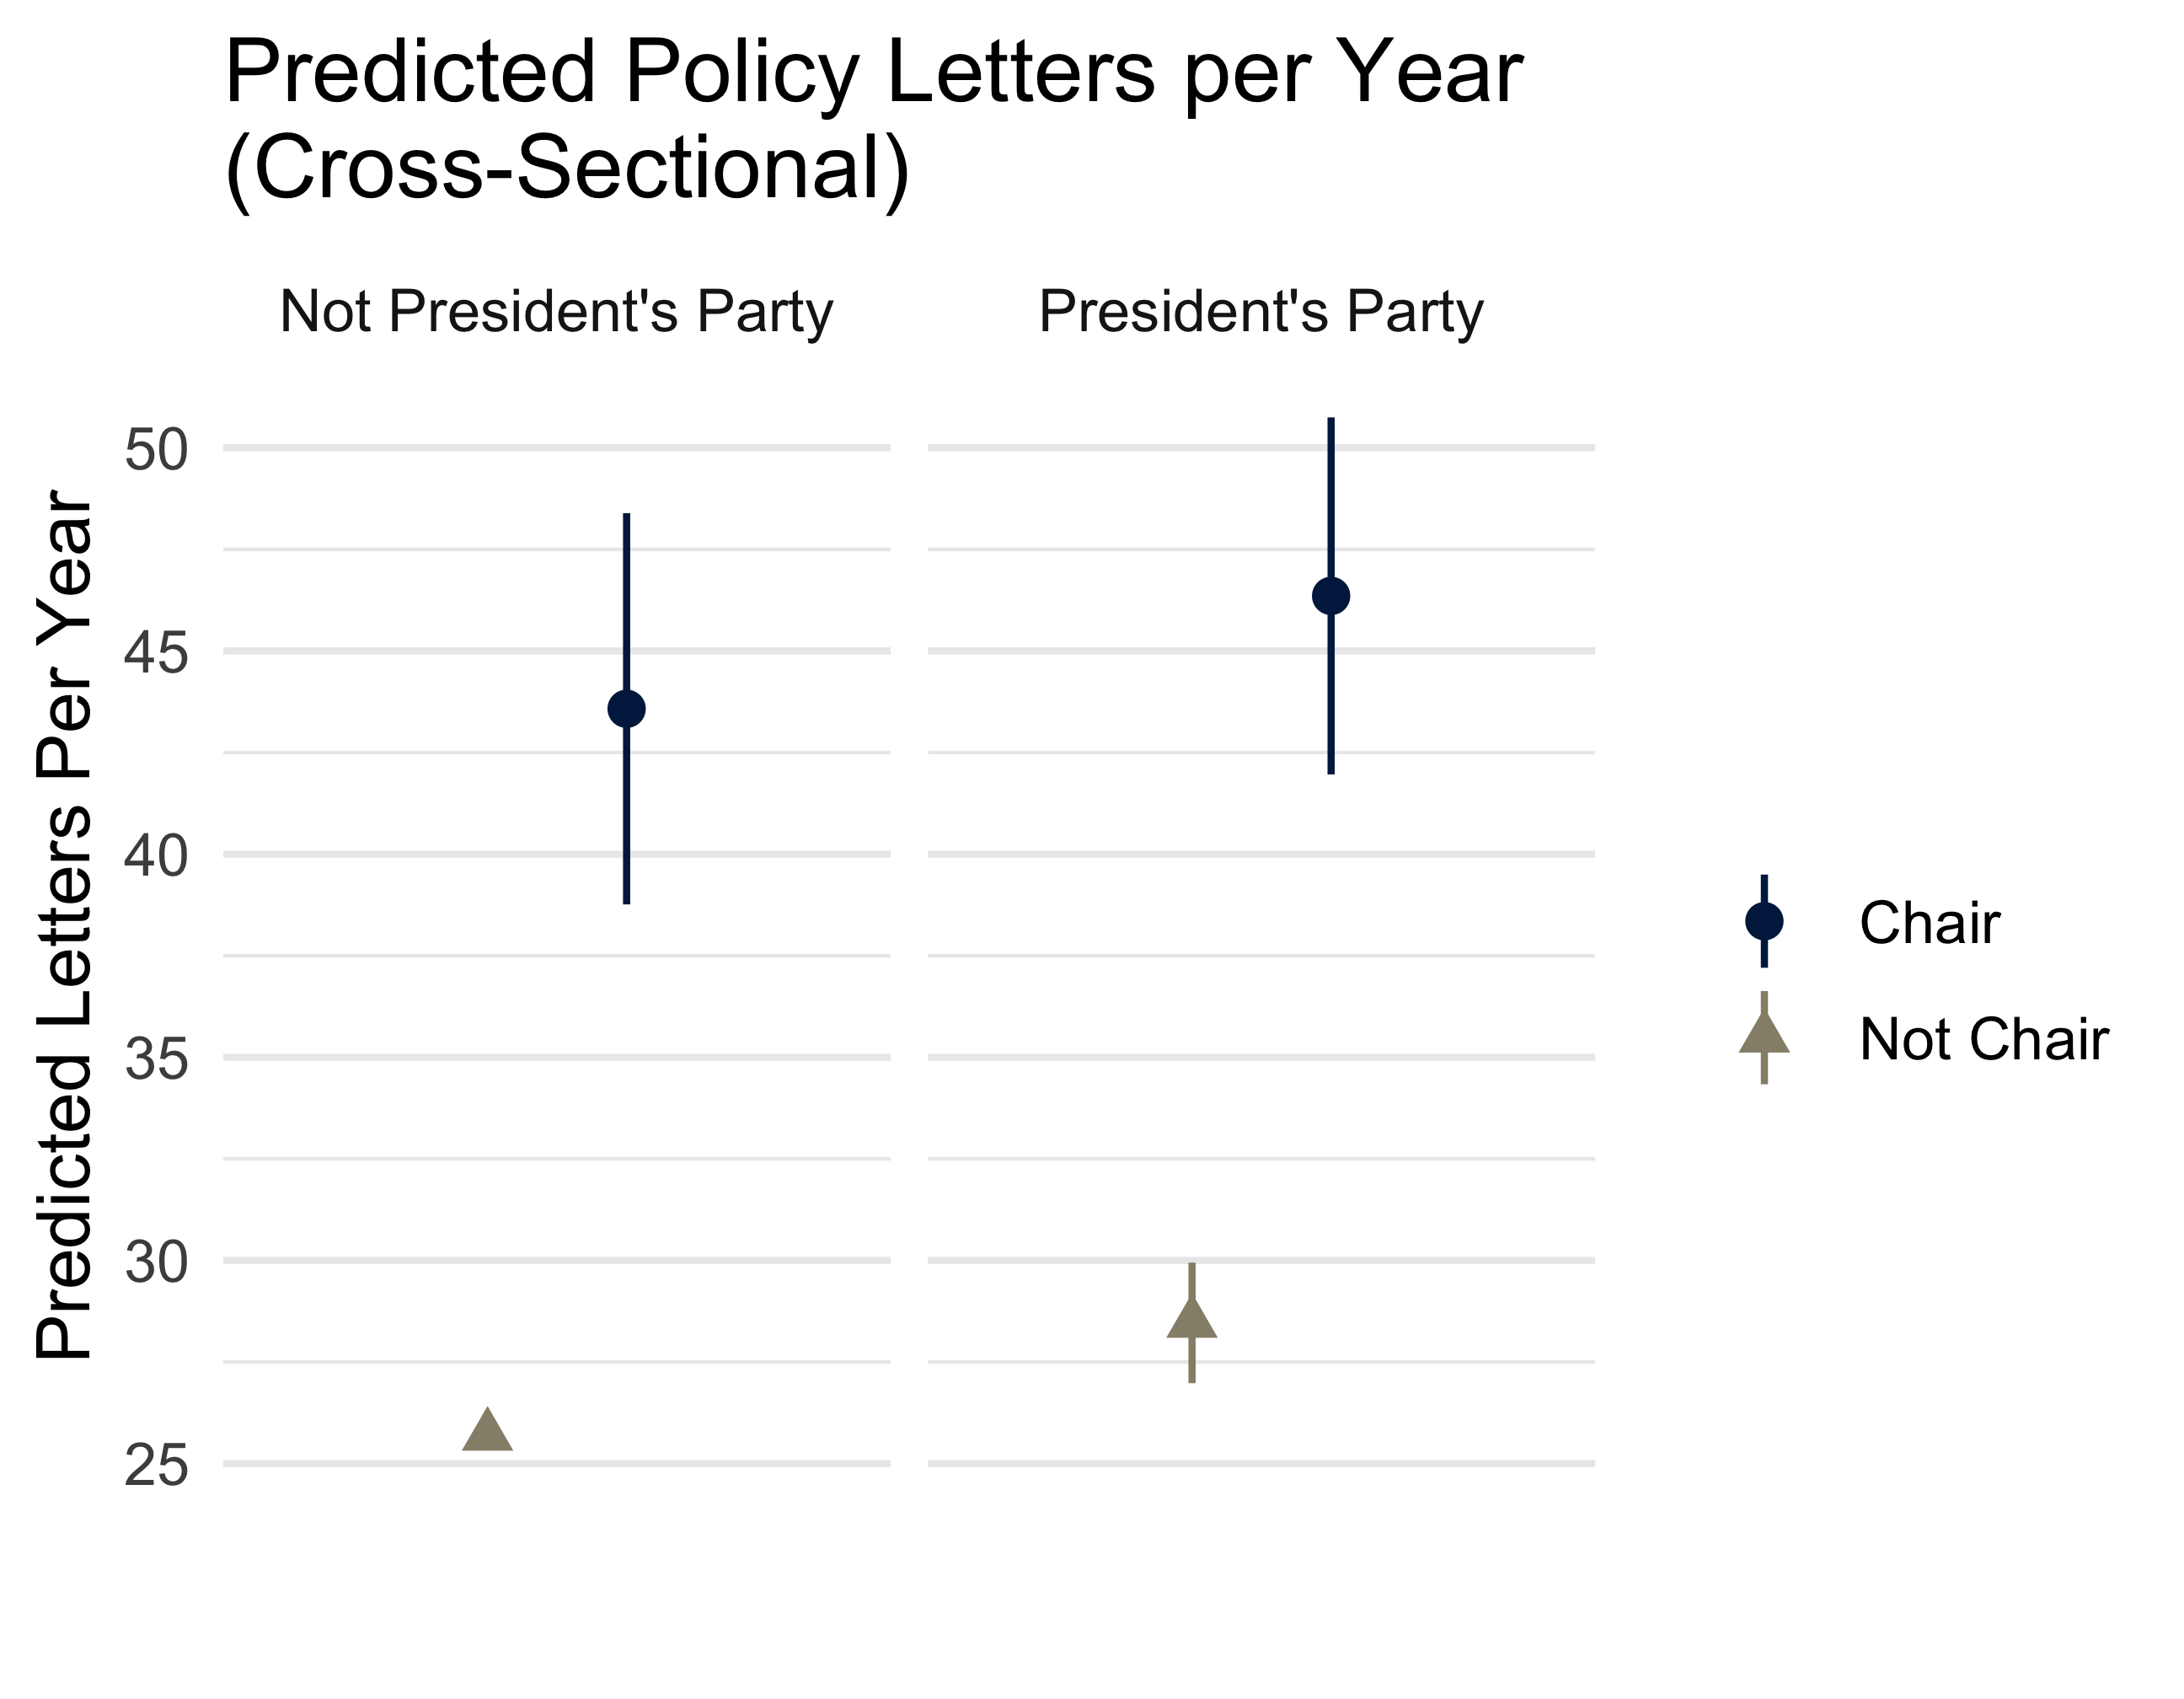
\includegraphics[width = .48\textwidth]{figs/m-policy-predicted-1} 
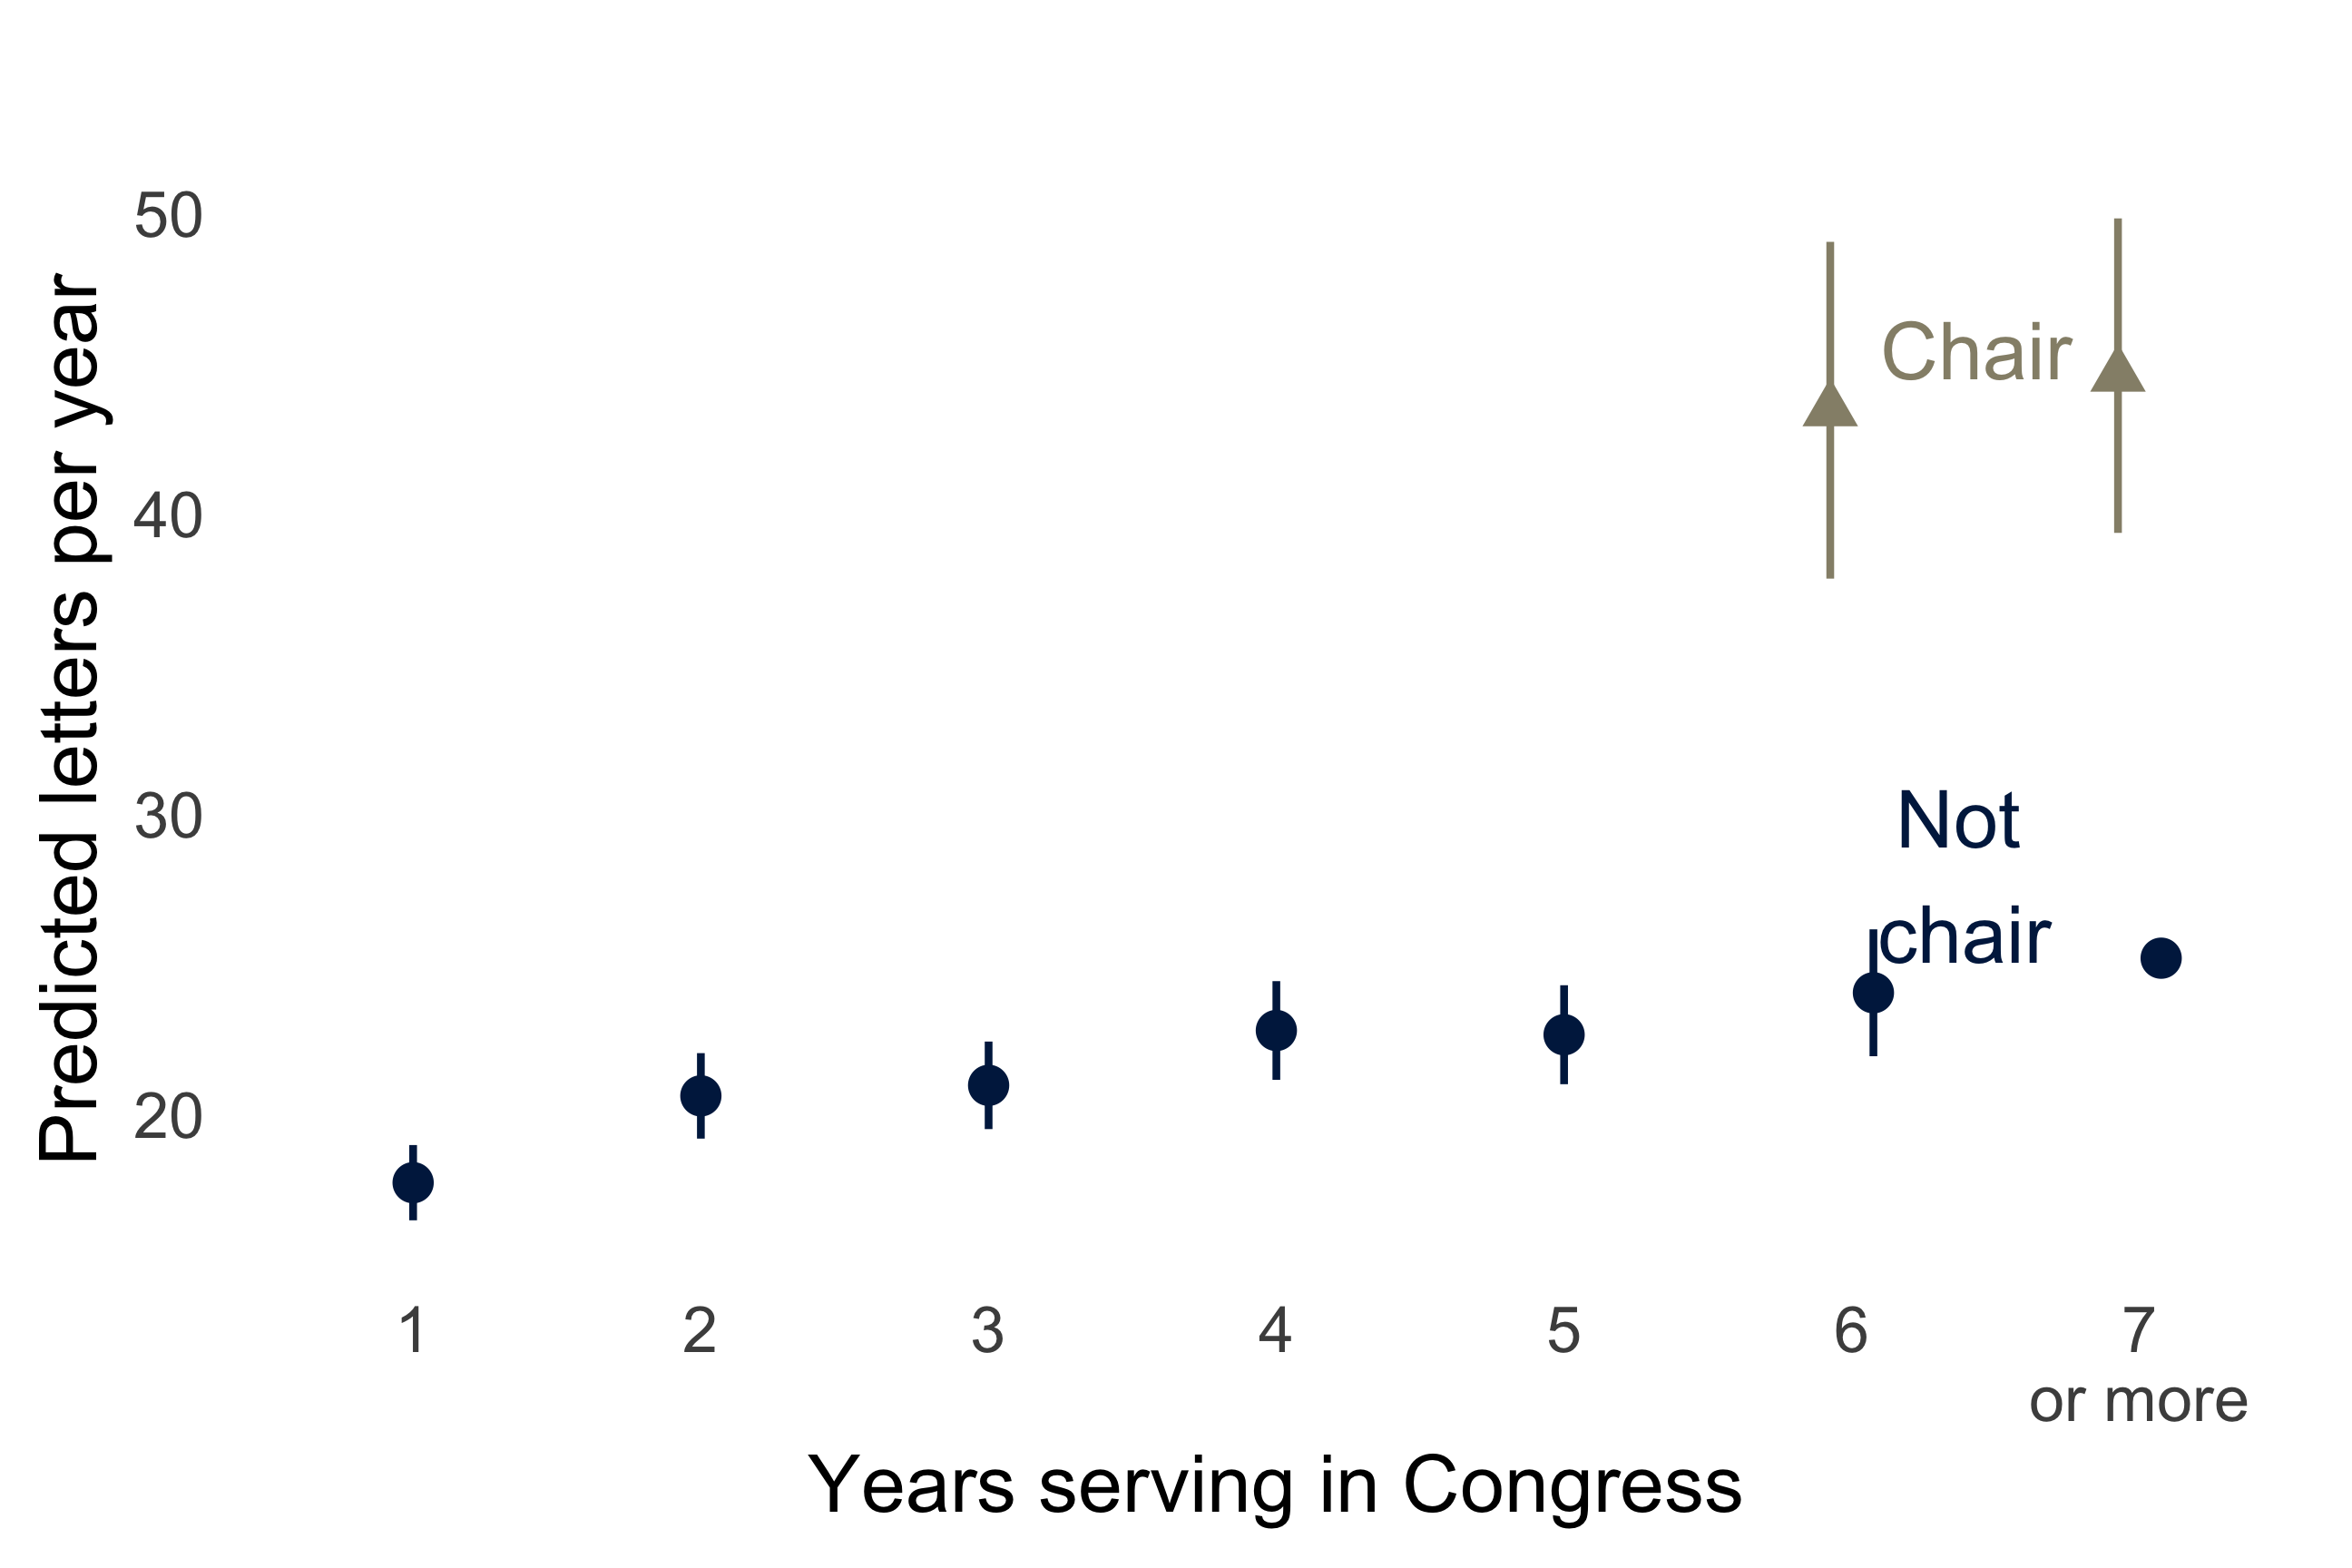
\includegraphics[width = .48\textwidth]{figs/m-policy-predicted-2} 
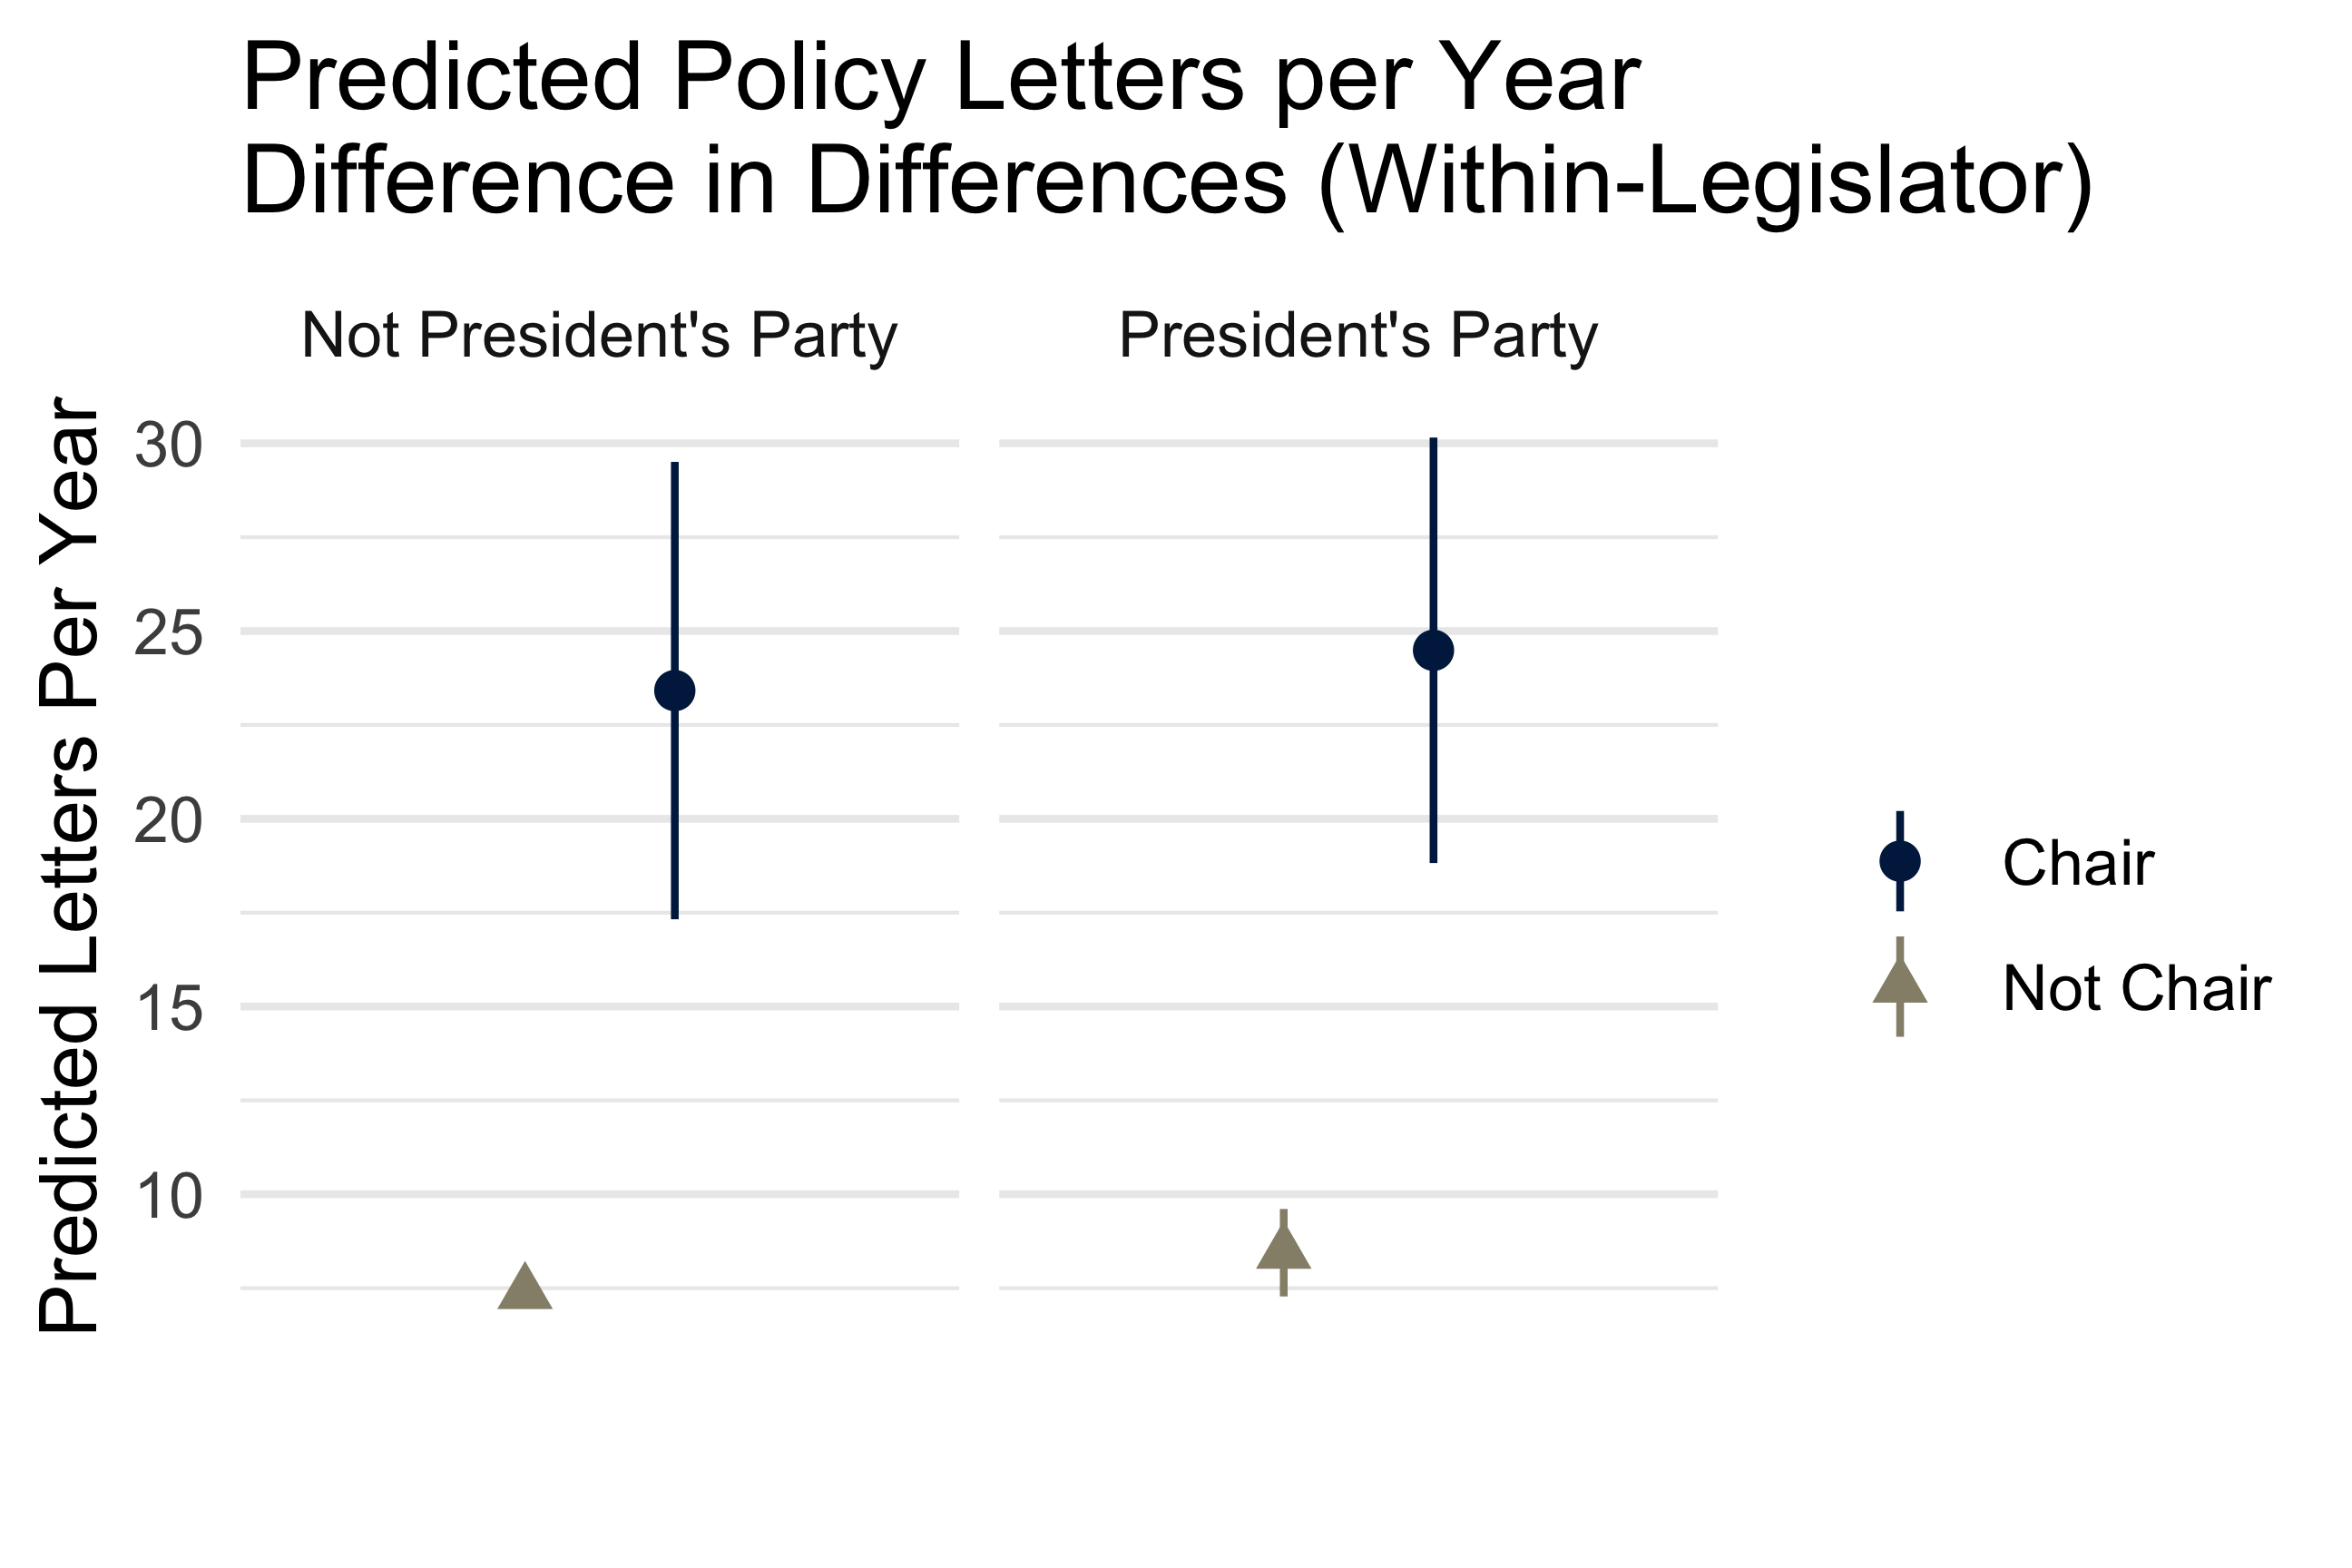
\includegraphics[width = .48\textwidth]{figs/m-policy-predicted-3} 
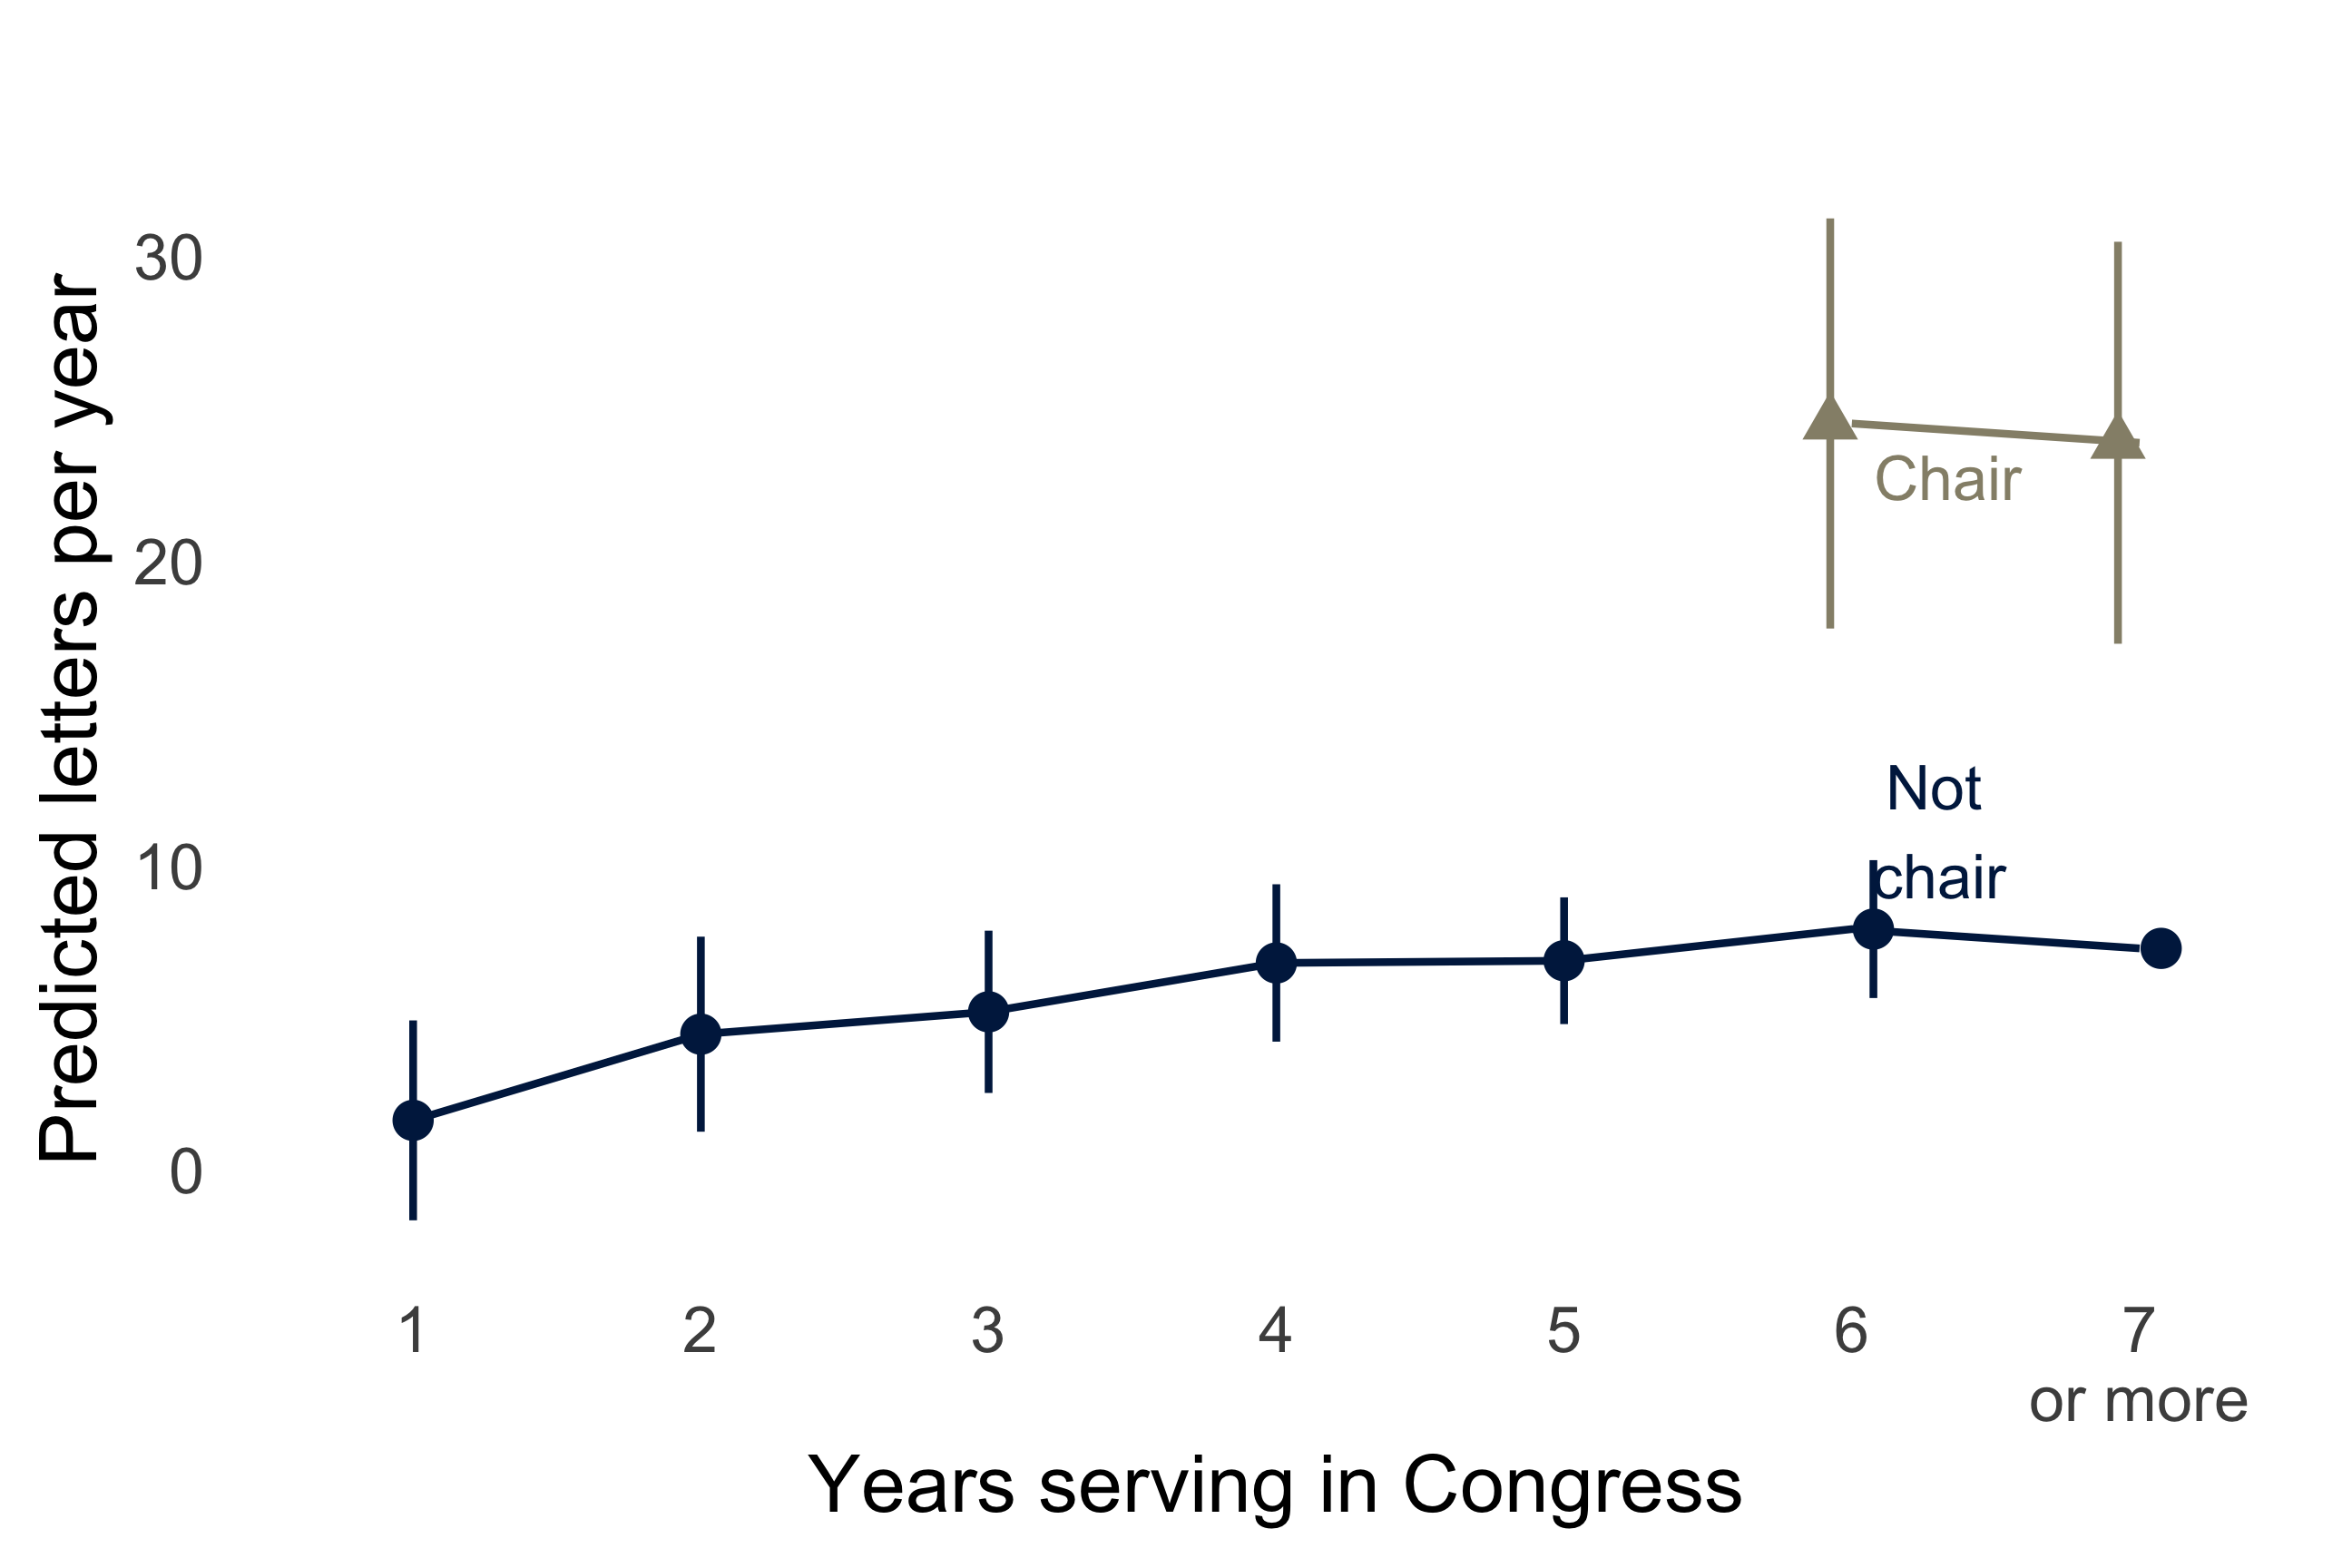
\includegraphics[width = .48\textwidth]{figs/m-policy-predicted-4} 

\end{figure}

\subsection{Within-District Models with Partisan Turnover} \label{s:appendix_models_district}


The main district-level models in Table \ref{t:models_district} of the paper focus on estimating the effect of legislator experience by leveraging turnover within districts. We compare the service that a district receives before and after electing a new legislator and in the following years as legislators gain experience in office.

As a robustness check, we replicate our within-district results using a subset of district-year-count observations where turnover in a district allows us to assess the partisanship of the prior member holding that seat. We interact an indicator of whether the prior member was of the ``same party" with all other indicators (i.e., whether the member is new, serving in years 1-6, or serving longer than 6 years). We compare the service that a district receives before and after electing a new legislator and in the following years, accounting for whether that member is of the same party. However, a structural constraint of the data means that this robustness check is limited to observations where turnover within a redistricting cycle gives us a measure of whether the legislator replaced a member of the same party or of another party. 

The table below accounts for redistricting by treating post-redistricting districts as new entities, not the same district as the one with the same number prior to redistricting (i.e., we do not count cases where a district elects someone of the same or different party as the district with the same number had before redistricting). Since some states completely re-number their districts, there is no way to be sure that a new District 4 has any relationship to the District 4 under the previous redistricting map (though it often may have significant overlap) without creating some spatial measure of the percent of shared census tracts, or something like that, which we do not attempt. 

Many NAs exist for the ``same party" variable because we only observe it when there is turnover *within* a redistricting cycle. Seats that do not turn over for an entire cycle (e.g., 2002-2012) are FALSE (``0") for ``new member" and have no value for ``same party." Other districts are NA until there is turnover. Thus, adding ``same party" causes significant data loss due to NAs. 
Specifically, we go from \textbf{7666 observations in Table \ref{t:models_district} to 2822 observations in Table \ref{t:models_district_party} when we include ``same party" in the models below.}

To measure turnover in the Senate where ``districts" have two members, we code ``same party" as FALSE if there is a change in the partisanship of a state's Senate delegation. This captures the parallel dynamic of single-member House districts. If there are two Democrats and one is replaced by a Republican, the ``same party" is FALSE. If there are two Democrats and a Democrat is elected, the ``same party" is TRUE. If there are a Democrat senator and a Republican senator representing a state, and the Democrat is replaced by a Republican, ``same party" is FALSE. As per the VoteView convention, Senate delegations are District ``0" (e.g., ``alabama\_0"). Split Senate delegations appear as ``Democratic Party;Republican Party" in the table below.

now on the number of contacts made from the representative of a particular state or district $i$ in a year $t$, $Y_{it}$. We again use a difference-in-differences approach to account for district-specific characteristics and over-time changes in how legislators provide constituency service. Specifically, we estimate regressions of the form: 


\begin{eqnarray}
Y_{it} & = & \beta_{1}\text{New Member}_{it}*\text{Same Party} + \sum_{s = 2}^{6} \beta_{s} \text{tenure}_{s[it]}*\text{Same Party} + \gamma_{i} + \delta_{t} + \epsilon_{it} \label{e:district1party} 
\end{eqnarray}

$\gamma_{i}$ is a district-specific fixed effect that accounts for each district's particular demographic characteristics, along with the levels of demand from district residents. $\delta_{t}$ is a year fixed effect that controls for common shocks. Our key result of interest, $\beta_{1}$, is the effect of a district electing a new representative. To understand how the effect of a new representative changes over time, we estimate district-level differences for a legislator's second ($\beta_{2}$) through sixth-year ($\beta_{6})$.\footnote{It is worth noting that this treatment is fundamentally different for a district than within-legislator variation. In each election, each district allows its incumbent to acquire another term or replaces her. This differs from within-legislator comparisons because legislators can only acquire more tenure or leave the chamber. A within-legislator analysis estimates the service provided by incumbents with more or less experience; it cannot estimate the impact of the choice of an incumbent or a new representative incumbent.} % TODO THIS FOOTNOTE IS REPETITIVE.

The first column of Table \ref{t:models_district_party} provides a simple difference-in-means for districts represented by a new member and legislators in their first six years in office. Districts represented by new legislators receive substantially lower levels of constituency service. On average, districts with a new representative have  fewer constituency service requests made on their behalf. The magnitude of this difference shrinks for districts represented by legislators in their second year It then reaches a relatively stable number for districts represented by legislators in their third through sixth years. %, with some slight evidence that legislators make more contacts in election years---the even-numbered years of tenure for the vast majority of legislators in our sample. 



\begin{table}[hbt!]
\caption{The Effect of Electing New Members on a District's Level of Constituency Service} \label{t:models_district_party}
\begin{minipage}{\textwidth}
\begin{center}
\small
\input{tables/models_district_party.tex}
\end{center}
\footnotetext{This table shows how constituent service at the district level changes over time. Model 1 is a cross-sectional comparison excluding district and year fixed effects. The second column is a district x year difference in differences model. Column 3 focuses is the diff-in-diff subsetted to legislators who survive their first election.}
\end{minipage}
\end{table}


To account for differences in district size, demographics, and demand for constituency service, the second column of Table \ref{t:models_district_party} estimates the difference-in-differences from Equation \ref{e:district1party}. In this specification, we see a large causal effect of a new member taking over: electing a new member causes a decrease in constituency service requests.
The effect of electing a new representative, however, dissipates quickly. This phenomenon--new legislators providing substantially fewer requests--persists when examining the House (Column 3) and the Senate (Column 4) separately, though results for the House are not stastically signicant in this restricted model. In short, new legislators make fewer contacts for their constituents than established legislators.  

\begin{figure}[hbt!]
\centering
\caption{Predicted Number of Total Letters per District) 2007-2018} \label{f:m-district-predicted-party}
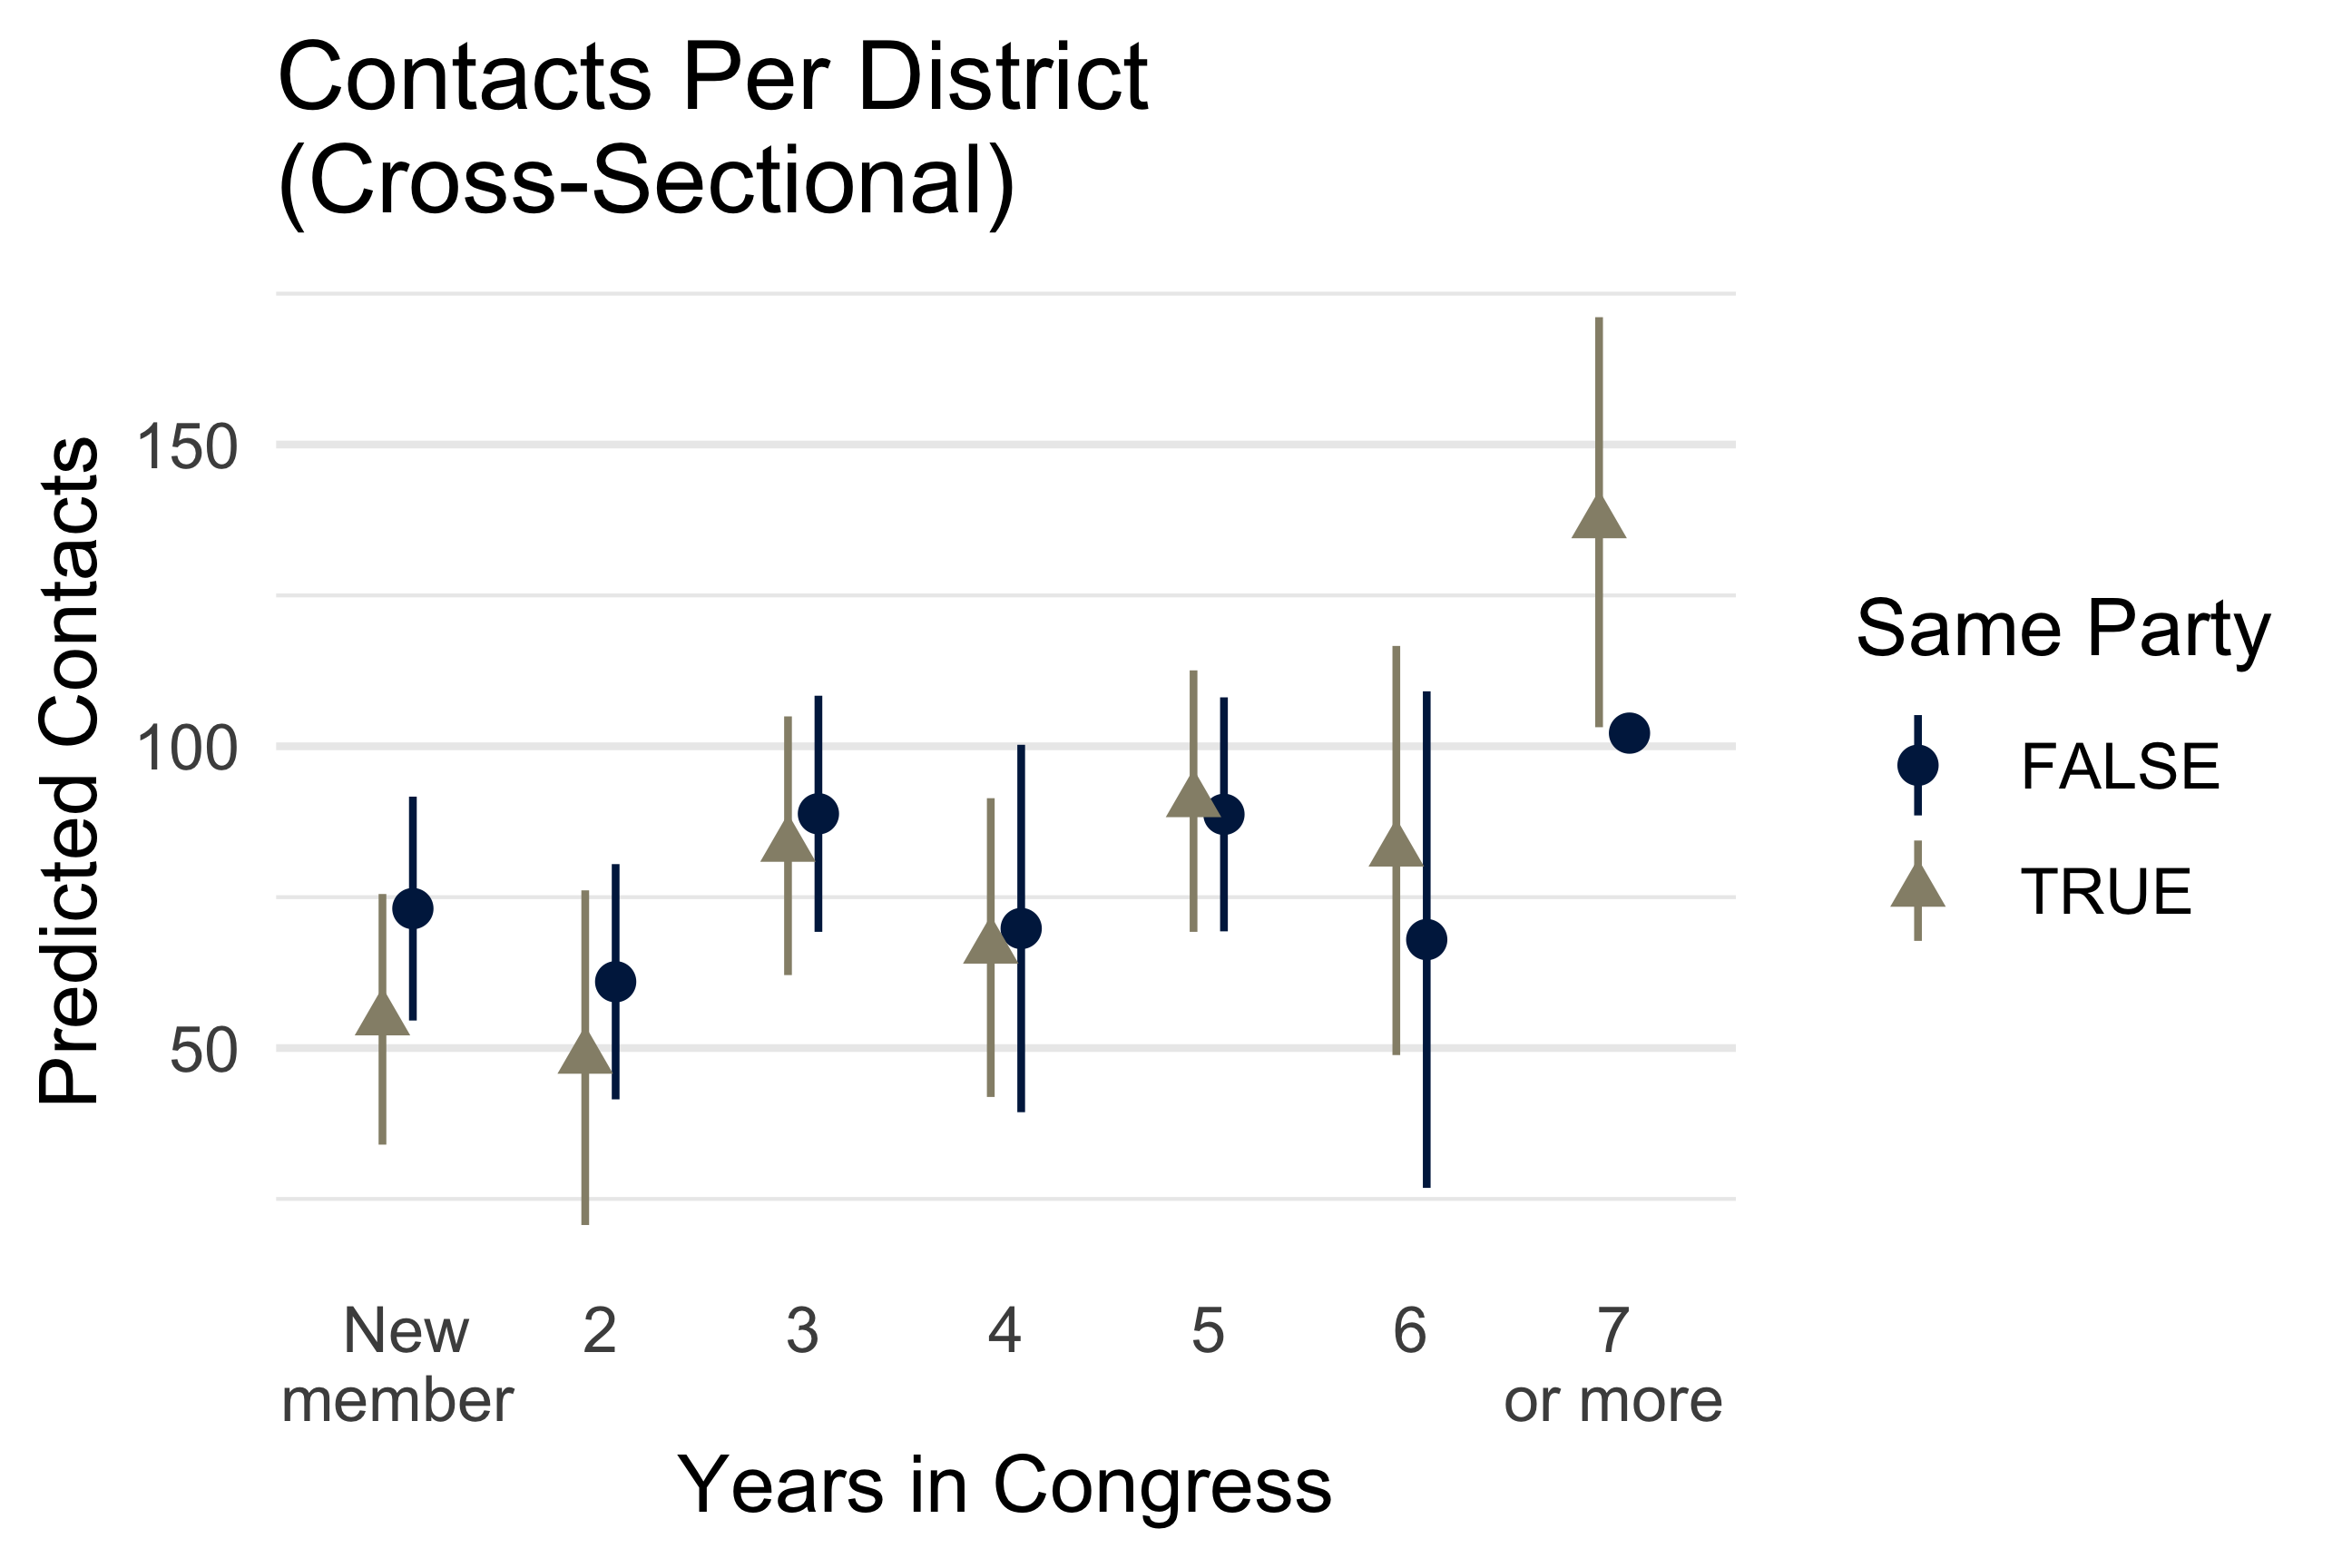
\includegraphics[width = .49\textwidth]{figs/m-district-predicted-2}
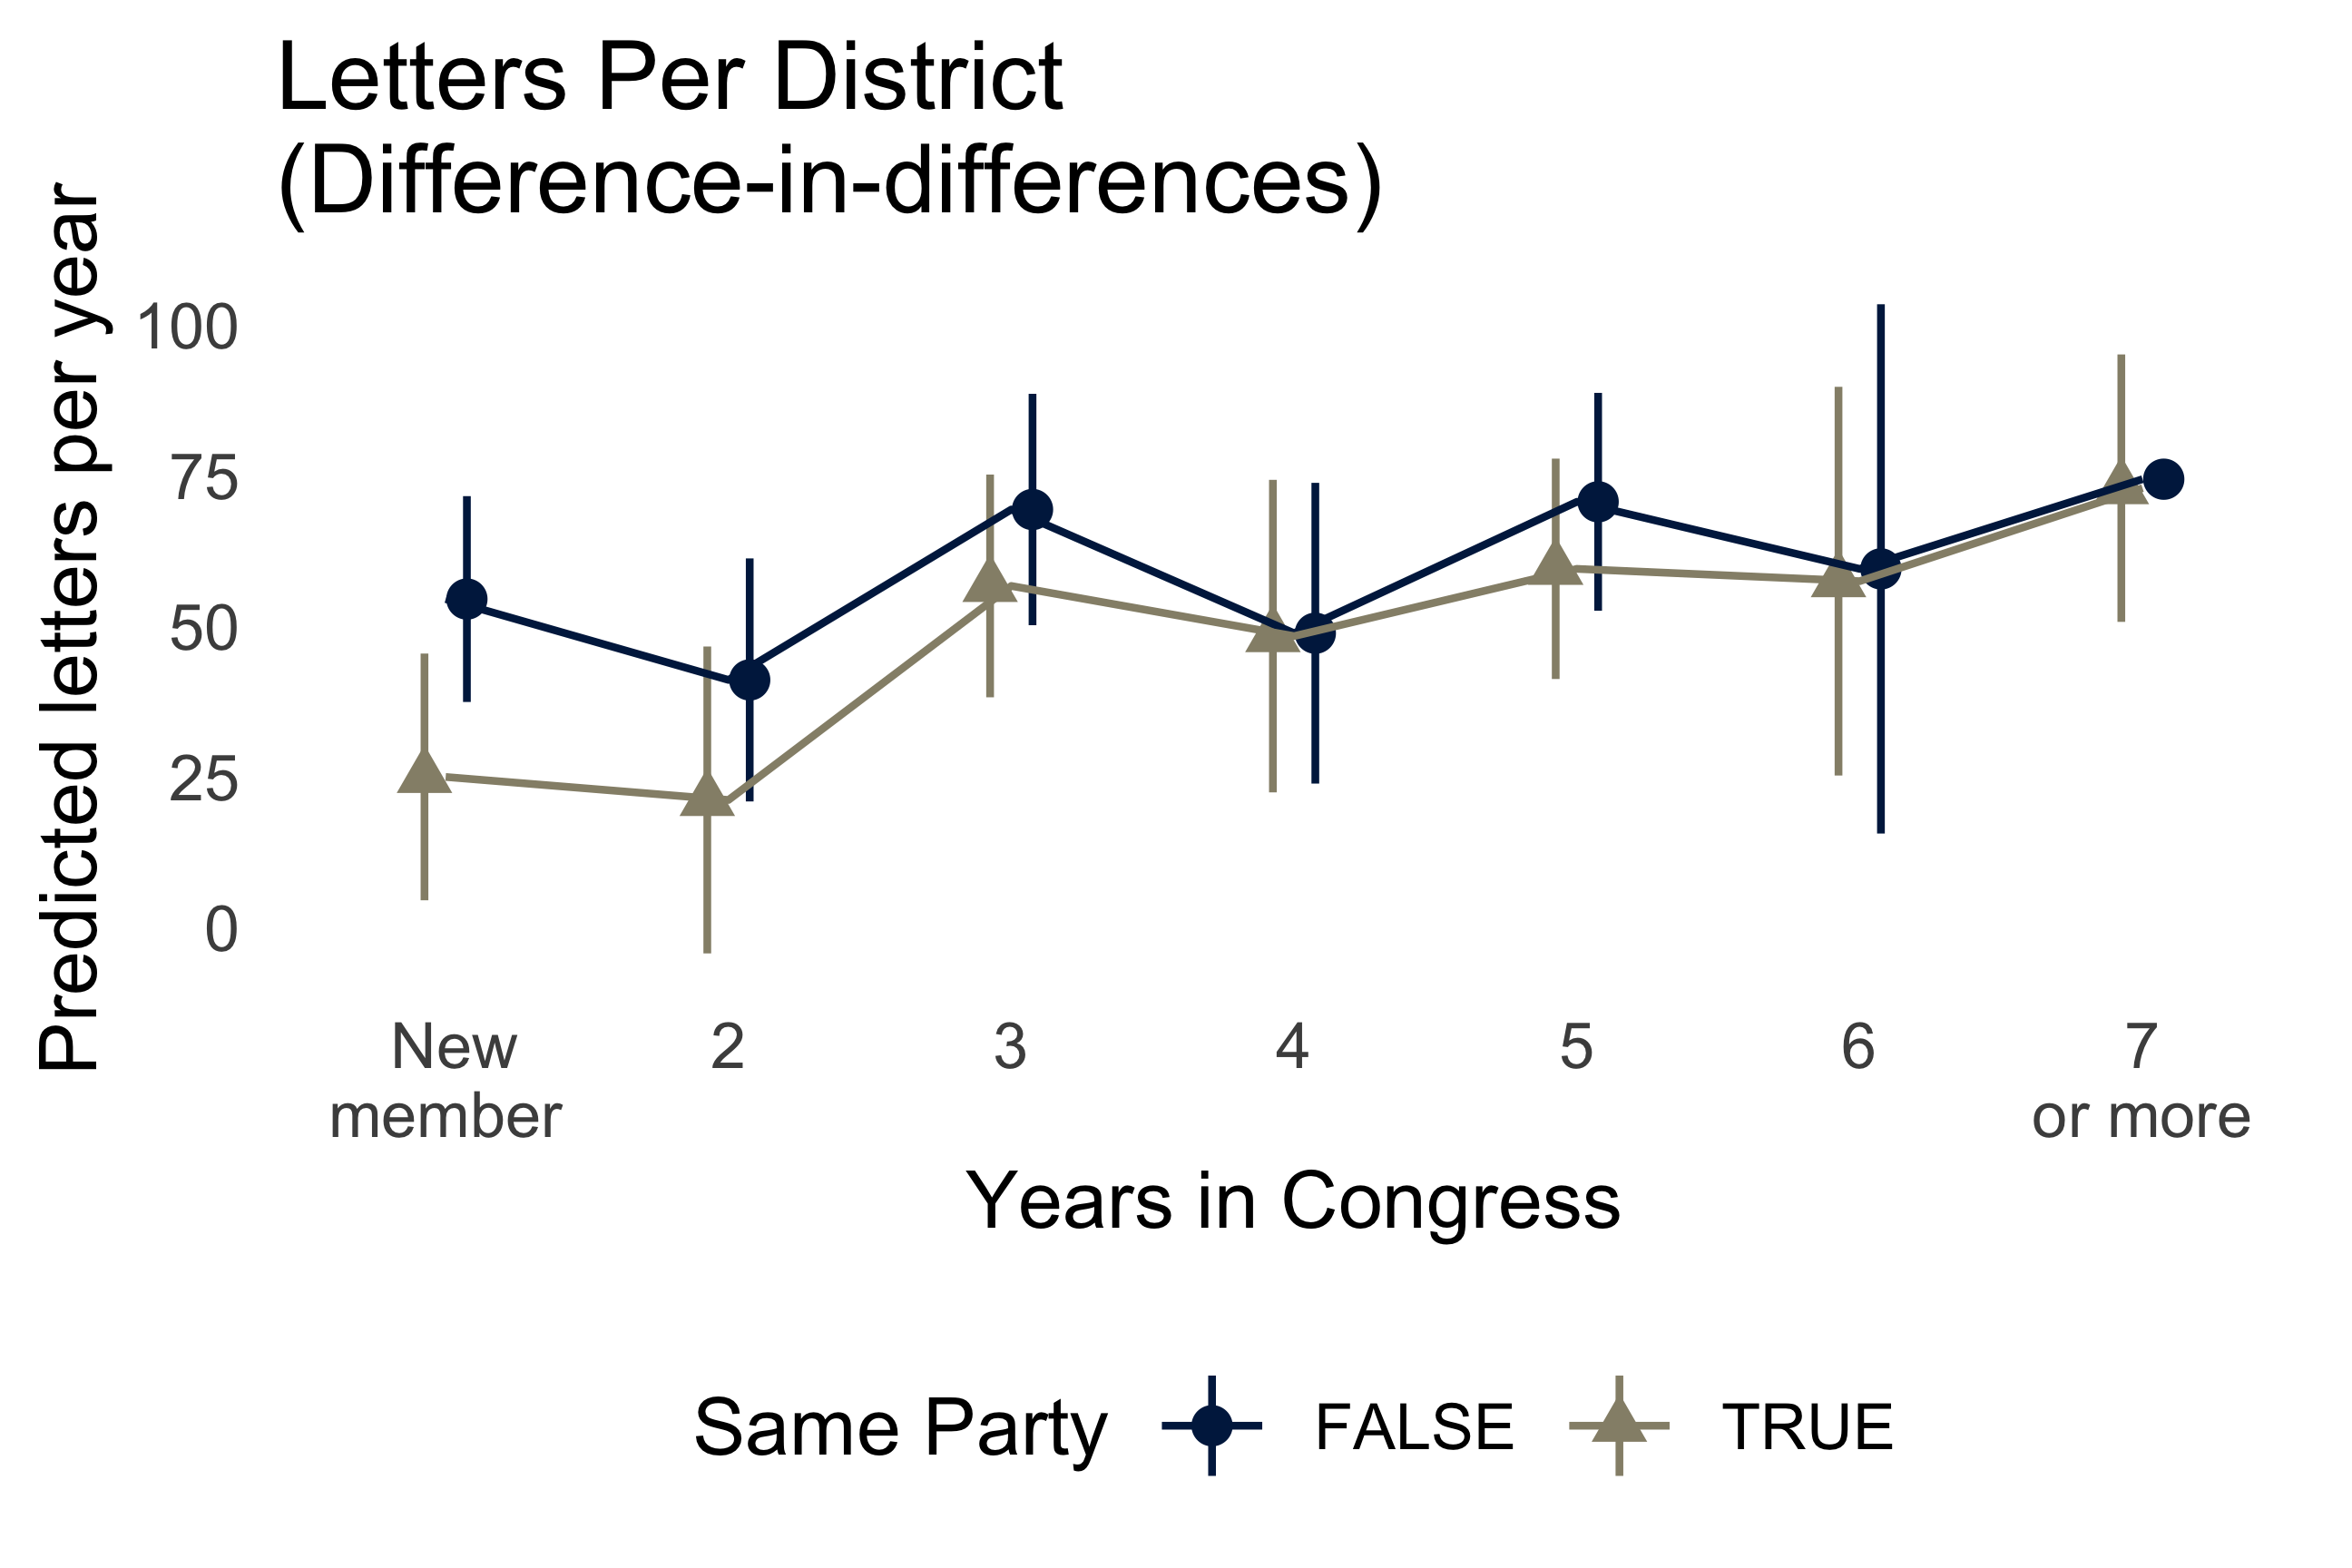
\includegraphics[width = .49\textwidth]{figs/m-district-predicted-4}
\end{figure}

Despite the increased uncertainty caused by the much smaller (and non-random) sample of districts where turnover allows us to measure the new “same party” variable, our main results (direction, statistical significance, and magnitude of effects) are largely the same: legislators contact the bureaucracy significantly less in their first two years in office, even holding district constant. Because the new models contain a large number of interaction terms, we present predictions at modal values in Figure \ref{f:m-district-predicted-party}.
Figure \ref{f:m-district-predicted-party} shows the predicted total number of letters per district per year by whether a district is represented by a new legislator and whether that legislator replaced a member of their same party (compared to counterfactuals where the same legislator has been serving for more than six years).\footnote{Predictions are based on a district-year pair where (1) the district's average annual contacts equaled the overall average, (2) the district's number of contacts with the agency equal the average received by that agency, (3) and the agency received an average number of letters.} 


